% Standalone journal-submission typesetting template (Journal of Automated Reasoning style).
\documentclass[11pt,a4paper]{article}
\usepackage[margin=26mm,headheight=15pt,headsep=8mm]{geometry}
\usepackage{fontspec}
\IfFontExistsTF{Liberation Serif}{%
  \setmainfont{Liberation Serif}%
}{%
  \setmainfont{Times New Roman}%
}
\IfFontExistsTF{Liberation Sans}{%
  \setsansfont{Liberation Sans}%
}{%
  \IfFontExistsTF{Latin Modern Sans}{%
    \setsansfont{Latin Modern Sans}%
  }{%
    \setsansfont{Helvetica}%
  }%
}
\IfFontExistsTF{DejaVu Sans Mono}{%
  \setmonofont[Scale=0.84]{DejaVu Sans Mono}%
}{%
  \IfFontExistsTF{Menlo}{%
    \setmonofont[Scale=0.81]{Menlo}%
  }{%
    \setmonofont[Scale=0.84]{Courier New}%
  }%
}
\usepackage{amsmath,amssymb,amsthm}
\usepackage{microtype}
\usepackage{setspace}
\setstretch{1.13}
\usepackage{longtable,booktabs,array,calc}
\newcounter{none}
\usepackage{needspace}
\usepackage{graphicx}
\usepackage{fancyhdr}
\usepackage[authoryear,round]{natbib}
\usepackage{xcolor}
\definecolor{linkblue}{HTML}{1F4463}
\PassOptionsToPackage{hyphens}{url}
\usepackage[unicode,colorlinks=true,allcolors=linkblue,bookmarksnumbered=true]{hyperref}
\usepackage{xurl}
\urlstyle{same}
\hypersetup{
  pdftitle={Pure-Kernel Verified Controller Synthesis, Fixed-Sample
Impossibility, and Calibrated Post-Selection Risk under Partial
Observation},
  pdfauthor={Degui Qian},
  pdfsubject={Interactive Theorem Proving, Partially Observed Stochastic Control, and Calibrated Risk Certification},
  pdfkeywords={interactive theorem proving; Lean 4; partially observable
Markov decision processes; safe controller synthesis; post-selection
inference; minimax regret}
}
\setlength{\parindent}{1.15em}
\setlength{\parskip}{2pt}
\setlength{\emergencystretch}{2.5em}
\setcounter{secnumdepth}{2}
\setcounter{tocdepth}{2}
\widowpenalty=10000
\clubpenalty=10000
\displaywidowpenalty=10000
\providecommand{\tightlist}{\setlength{\itemsep}{2pt}\setlength{\parskip}{0pt}}
\providecommand{\passthrough}[1]{#1}
\pagestyle{fancy}
\fancyhf{}
\fancyhead[L]{\footnotesize Qian: Pure-Kernel Verified Controller Synthesis}
\fancyhead[R]{\footnotesize Calibrated Post-Selection Risk under Partial Observation}
\fancyfoot[C]{\small\thepage}
\renewcommand{\headrulewidth}{0.25pt}
\fancypagestyle{plain}{\fancyhf{}\fancyfoot[C]{\small\thepage}\renewcommand{\headrulewidth}{0pt}}
\begin{document}
\thispagestyle{plain}
\begin{center}
{\fontsize{18.5}{23}\selectfont\bfseries Pure-Kernel Verified Controller
Synthesis, Fixed-Sample Impossibility, and Calibrated Post-Selection
Risk under Partial Observation\par}
\vspace{11pt}
{\large Degui Qian\par}
\vspace{3pt}
{\small Independent Researcher\par}
\vspace{5pt}
{\small November 2026\par}
\end{center}
\vspace{4pt}
\begin{abstract}
\noindent Executable controller synthesis for partially observed
stochastic systems faces three verification gaps: qualitative shields
assume exact transition supports whereas data-driven pipelines select
abstractions from finite samples; continuous belief compressions can
erase hidden safety hazards; and mechanized rational dynamic-programming
proofs often rely on compiler-trusted evaluation axioms. We close these
gaps in an end-to-end mathematical and Lean 4 formalization whose proof
terms depend solely on Lean's three standard logical axioms. First,
without requiring a finite enumeration of the observation type, we
connect positive-mass posterior supports and all-time viability to a
sound-and-complete computable finite-memory controller synthesizer
achieving almost-sure infinite-trajectory safety. Second, after proving
that no randomized fixed-sample black-box test can uniformly certify
exact zero transition leakage, we combine prior structural supports with
a computable rational risk oracle on a single simultaneous
row-calibration event---eliminating candidate-count union penalties,
bounding false acceptance of over-budget controllers by \(\alpha_N\),
and bounding unconditional joint acceptance-and-failure by
\(\alpha_N + (1-\alpha_N)\beta\) (distinct from post-acceptance
conditional risk on rare miscalibrated samples). Third, we characterize
measurable binary-observation belief quotients via closed test spaces
and establish exact prepaid fault-discrimination and randomized minimax
regret (\(3/128 < 1/32\)) via greatest-common-divisor-free integer
dynamic programming verified purely inside Lean's kernel.
\end{abstract}
\vspace{4pt}
\noindent{\small\textbf{Keywords:} interactive theorem proving; Lean 4;
partially observable Markov decision processes; safe controller
synthesis; post-selection inference; minimax regret}
\vspace{12pt}

\section{Introduction: bridging structural safety, statistical
calibration, and kernel
trust}\label{introduction-bridging-structural-safety-statistical-calibration-and-kernel-trust}

Designing and certifying autonomous controllers for partially observed
stochastic systems requires reconciling three traditions whose
foundational assumptions rarely align. In formal methods, supervisory
control \citep{ramadgeWonham1987, tabuada2009, cassandrasLafortune2021},
probabilistic model checking
\citep{baierKatoen2008, kwiatkowska2011, dehnert2017}, and shield
synthesis for reinforcement learning under partial observability
\citep{chatterjee2016, alshiekh2018, junges2021, carr2023} construct
finite-memory strategies that enforce safety or almost-sure reachability
invariants across unbounded horizons. Crucially, qualitative
support-based synthesis assumes an \emph{exact} relational specification
of which state transitions carry strictly positive probability. In
statistical machine learning and robust control, by contrast, transition
kernels are unknown and must be estimated from finite sample
trajectories
\citep{kearnsSingh2002, strehl2009, nilimElGhaoui2005, wiesemann2013},
while practitioners routinely use the same training dataset both to
select a coarse observation abstraction
\citep{ravindranBarto2004, ferns2004} and to bound downstream deployment
failure---creating a classic post-selection inference hazard
\citep{berk2013, mayo2018}. Meanwhile, in interactive theorem proving
\citep{nipkowPaulsonWenzel2002, bertotCasteran2004, mouraUllrich2021},
recent formalizations have mechanized foundational measure-theoretic
Markov processes and fully observed tabular dynamic programming
\citep{hoelzl2017, vajjha2021, schaeffelerAbdulaziz2023}, yet concrete
rational horizon evaluations for partially observed belief trees often
suffer severe kernel reduction blowup from repeated
greatest-common-divisor normalization, tempting developments to
introduce compiler-trust evaluation axioms \citep{boespflug2011}.

When these three layers are left disconnected, subtle soundness bugs
slip between their interfaces. Consider four concrete failure modes that
arise in naive combinations of synthesis, abstraction, and statistical
testing:

\begin{enumerate}
\def\labelenumi{\arabic{enumi}.}
\tightlist
\item
  \emph{Reference-history reachability circularity and dead-end
  prefixes.} On any fixed positive-mass action--observation history
  \(g\), the numerical state posterior is determined by \((p_0, P, q)\)
  and the recorded pairs in \(g\)
  \citep{astrom1965, smallwoodSondik1973, kaelbling1998}, yet
  \emph{which histories \(g\) receive positive probability} depends on
  the deployed policy \(\pi\). Proving that a synthesized policy visits
  only certified state--action pairs on histories reachable under a
  \emph{pre-fixed} reference policy fails if deploying the new
  controller shifts positive probability onto previously unvisited
  observation branches. Conversely, verifying that an action is locally
  certified at the present step does not imply that the resulting
  support admits any safe continuation at subsequent steps.
\item
  \emph{The illusion of black-box zero-risk certification.} Because
  support-based shields require exact transition supports
  \(R(x,a,z) \iff P(x,a)(z) > 0\), it is tempting to certify
  \(P(x,a)(x^*) = 0\) empirically after observing zero visits to a
  hazardous state \(x^*\) across \(N\) independent trials. Yet without
  an independently justified minimum positive transition margin, an
  adversarial or unmodeled contamination rate
  \(\varepsilon \in (0, 1/N)\) produces an all-safe training record with
  high probability \((1-\varepsilon)^N\) while breaking infinite-horizon
  almost-sure safety.
\item
  \emph{Post-selection optimism and candidate-count inflation.} When an
  algorithm scans a family of candidate coarse observation maps
  \(q_1, \dots, q_m\) on empirical transition data and deploys the first
  abstraction passing a defect threshold, conditioning naively on
  acceptance invalidates finite-sample concentration, whereas taking a
  union bound over all \(m\) candidate abstractions inflates sample
  complexity even though all abstractions project the \emph{same}
  underlying state--action transition rows. Moreover, even on standard
  Borel spaces where exact predictive compression succeeds
  \citep{crutchfieldYoung1989, shaliziCrutchfield2001, barnettCrutchfield2015},
  two latent beliefs that agree on every future observation test can
  assign opposite values to hidden-state safety predicates.
\item
  \emph{Resource-gated fault ambiguity and compiler-trusted reflection.}
  In cyber-physical and fault-tolerant register architectures, probing
  whether faults act locally on a single dispatched unit or globally
  across backup units consumes prepaid operational budget. Under strict
  per-step prepayment, insufficient budget renders distinct fault
  mechanisms observationally indistinguishable; at intermediate
  horizons, deterministic controllers hit discrete payoff-lattice
  barriers that pre-committed randomized controllers strictly beat
  \citep{vonNeumann1928, wald1950, savage1951}. Certifying exact
  rational minimax regret across full observation trees via
  computational reflection \citep{boutin1997, gregoireMahboubi2005}
  forfeits pure-kernel assurance if rational arithmetic triggers
  compiler-trusted evaluation.
\end{enumerate}

This article presents a unified mathematical theory and pure-kernel Lean
4 formalization \citep{mouraUllrich2021, mathlib2020} centered on
executable controller synthesis with exact probabilistic semantics and
machine-checked post-selection deployment risk. Every theorem, witness,
synthesizer, statistical risk oracle, and minimax regret bound reported
here has its proof terms checked by Lean 4 (version 4.33.1) over
Mathlib, passing an environment-wide axiom audit across all 1,030
declaration-defining modules (within the 1,051-module compiled library)
that restricts transitive dependencies exclusively to Lean's three
standard logical axioms---propositional extensionality
(\texttt{propext}), classical choice (\texttt{Classical.choice}), and
quotient soundness (\texttt{Quot.sound}) \citep{carneiro2019}---with
zero incomplete proofs (\texttt{sorryAx}) and zero compiler-trust
evaluation axioms (\texttt{Lean.ofReduceBool} /
\texttt{native\_decide}). All mathematical definitions, analytical
proofs of Theorems 1--6 and Theorem 7.1, and explicit strategy
evaluations are presented in Sections 2--6 and Appendix A.1--A.6, while
full-menu optimality across all seven-action trees in Theorem 7.2 is
established as a computer-assisted pure-kernel dynamic-programming proof
independently reproducible via both Lean (\texttt{lake\ env\ lean}) and
our zero-dependency standalone Python verifier
(\texttt{verify\_standalone.py}).

Our main contributions form a tightly integrated chain across four
levels:

\begin{itemize}
\tightlist
\item
  \textbf{Exact trace-support viability, König quantifier exchange, and
  executable synthesis (Sections 2--3).} For finite state spaces \(X\),
  finite action sets \(A\), and arbitrary observation types \(Y\)
  (requiring no finite enumeration of \(Y\) at the interface, since
  \(q(X)\) has size at most \(|X|\)), Theorem 1 proves that on every
  coarse history of positive probability under an arbitrary causal
  policy \(\pi\), the exact posterior support coincides with the
  combinatorial trace-support recursion \(S_n(g)\), yielding a
  non-circular equivalence between backward support viability
  \(V(0, T, S_0(y))\) and existence of a causal policy achieving zero
  uncertified occupancy \(\nu_n^\pi(C_n^c) = 0\) across \([0,T)\).
  Theorem 2 establishes a König-type compactness equivalence
  \citep{konig1927} for time-inhomogeneous systems: arbitrarily long
  finite-horizon zero-uncovered policies exist if and only if a
  \emph{single} causal policy \(\pi_\infty\) certifies all times
  \(n \in \mathbb{N}\) simultaneously (contrasted with countable-state
  countdown failure). Theorem 3 bounds Kleene winning-arena
  stabilization by \(2^{|X|} - 1\) rounds
  \citep{tarski1955, aubinCellina1984, aubin1991}, connects closed-loop
  substochastic killed matrix powers
  \(\mathbf{1}_{\widetilde{K}}^\top Q_K^T \widetilde{\mu}_0\)
  \citep{darrochSeneta1965, seneta1981, collet2013} to the Kolmogorov
  infinite-trajectory safety probability
  \(\mathbb{P}(\forall n \in \mathbb{N},\, X_n \in K)\)
  \citep{kallenberg2021}, and proves soundness and completeness of the
  purely computable synthesizer \texttt{synthesize} returning
  \texttt{Option\ (Program\ X\ Y\ A)}.
\item
  \textbf{Fixed-sample impossibility and candidate-free calibrated
  post-selection risk (Section 4).} Theorem 4 proves that for any fixed
  sample size \(N \ge 1\), significance level \(\alpha \ge 0\), and
  \emph{randomized} certification kernel
  \(\psi : \{0,1\}^N \to \Delta(\{\mathrm{true}, \mathrm{false}\})\),
  uniform \(\alpha\)-validity over positive hazard rates \(p \in (0,1)\)
  forces \(\mathbb{P}_0(\psi = \mathrm{true}) \le \alpha\) at \(p = 0\)
  \citep{leCam1973, tsybakov2009}. Pairing prior structural supports
  \((I_0 = \operatorname{supp}(p_0),\, R = \operatorname{supp}(P))\)
  with per-row empirical transitions, Theorem 5 separates sample-free
  infinite-horizon safety in \(K\) from calibrated finite-horizon risk
  on the joint training--selected-deployment law
  \(J(\omega, h) = \mu(\omega) K_{s(\omega)}(h)\), verifying
  \texttt{NoisyFiniteRiskOracle} across \emph{all} candidate
  abstractions \(q_0, \dots, q_{m-1}\) on a single row-calibration event
  \(G_u\) \citep{hoeffding1963, mcdiarmid1989, pinsker1964} via Markov
  pushforward contractivity \citep{dobrushin1956, csiszar1975} without
  \(m\)-union penalties. Exact integer-binomial operating curves
  (\(u_N \propto N^{-1/2}\)) and a \(12\)-state multi-abstraction
  benchmark quantify compact \(4\)-state controllers and
  \(72\times\)--\(147\times\) faster macro-reference verification
  against microscopic \(\widehat{P}\) evaluation.
\item
  \textbf{Binary-observation belief quotients vs.~prepaid
  fault-mechanism minimax regret (Sections 5--6).} On standard Borel
  state spaces \(X\)
  \citep{giry1982, bertsekasShreve1978, hernandezLerma1996} with
  deterministic binary observation \(q: X \to \{0,1\}\), Theorem 6
  proves that the regular posterior-belief kernel descends through
  \(c_q(b) = b(q^{-1}\{1\}) \in [0,1]\) to a unique Markov quotient
  kernel \(\bar{K}\) (concentrating updated coordinates on \(\{0,1\}\))
  \citep{burkeRosenblatt1958, kemenySnell1960, larsenSkou1991, givanDeanGreig2003}
  if and only if \texttt{ClosedTests} holds, while demonstrating that
  predictive sufficiency can erase hidden-state safety invariants
  \citep{jaeger2000, littmanSuttonSingh2001}. Under a non-replenished
  prepayment wallet \(B\) \citep{altman1999, conantAshby1970, pearl2009}
  comparing serial local faults (\(S\)) against global correlated faults
  (\(G\)), Theorem 7 establishes exact three-step distinguishability
  \(\Delta_{3,B} = r^2(1-r)\mathbf{1}_{B \ge c}\)
  \citep{blackwell1953, coverThomas2006} and proves via Bayes--minimax
  duality \citep{bellman1957, blackwell1965, savage1951} that at
  \((1/2, 3, 2, 1, 1/4, 1)\) pre-run randomization strictly beats
  deterministic strategies (\(R^* = 3/128 < 1/32\)).
\item
  \textbf{Pure-kernel formalization architecture, GCD-free integer DP,
  and reproducible audit (Section 7).} We detail our
  computable-to-measure semantic bridge, show how unnormalized
  integer-weighted beliefs (\texttt{UBelief}) and dyadic scaling
  (\texttt{csolveInt}, \texttt{csourceInt}) eliminate \texttt{Nat.gcd}
  normalization so full-menu POMDP values verify inside Lean's kernel
  via \texttt{decide} without compiler-trust axioms, report reproducible
  wall-clock verification times and module audit counts, and compare
  interfaces and guarantees against Isabelle/HOL, Coq/Rocq, and POMDP
  shielding tools
  \citep{affeldt2014, eberl2015, hoelzlNipkow2012, hoelzl2017, vajjha2021, junges2021, carr2023, schaeffelerAbdulaziz2023}.
\end{itemize}

\section{Trace-support viability and compact quantifier exchange under
partial
observation}\label{trace-support-viability-and-compact-quantifier-exchange-under-partial-observation}

\subsection{Microscopic and coarse path laws without reference-policy
circularity}\label{microscopic-and-coarse-path-laws-without-reference-policy-circularity}

Let \(X\) be a finite state space, \(A\) be a finite nonempty action
set, and \(Y\) be an arbitrary observation type equipped with a
deterministic observation map \(q: X \to Y\). Crucially, we do
\emph{not} require a finite enumeration of \(Y\) at the specification or
theorem-proving interface: because \(X\) is finite and \(q\) is
deterministic, the effective image \(q(X) \subseteq Y\) realized with
positive probability has cardinality at most \(|X|\), allowing Lean
formalizations to instantiate \(Y\) directly with ambient infinite types
(such as \texttt{Nat}, \texttt{String}, or product records) without
finite-subtype wrapper boilerplate. Time-inhomogeneous stochastic
dynamics are specified by an initial state probability mass function
(PMF) \(p_0 \in \Delta(X)\) and a sequence of transition kernels
\(P_n: X \times A \to \Delta(X)\) for \(n \in \mathbb{N}\)
\citep{paz1971, puterman1994}. At each step \(n\), a task-specific
safety or operational specification is represented by a binary
state--action certification relation \(C_n \subseteq X \times A\); a
pair \((x,a) \in C_n\) is \emph{certified} at step \(n\), and
\((x,a) \in C_n^c := (X \times A) \setminus C_n\) is \emph{uncertified}
(or \emph{uncovered}).

A \emph{coarse causal history} of length \(n\) records the initial
observation together with the sequence of applied actions and received
observations:
\[\mathcal{H}_0 := Y, \qquad \mathcal{H}_{n+1} := \mathcal{H}_n \times (A \times Y).\]
Correspondingly, a \emph{microscopic history} \(h_n \in \mathcal{M}_n\)
records the full state--action trajectory \(\mathcal{M}_0 := X\) and
\(\mathcal{M}_{n+1} := \mathcal{M}_n \times (A \times X)\), projecting
onto coarse histories via \(\Pi_0(x_0) := q(x_0)\) and
\(\Pi_{n+1}(h_n, (a_n, x_{n+1})) := (\Pi_n(h_n), (a_n, q(x_{n+1})))\),
with terminal state \(\mathrm{last}_0(x_0) := x_0\) and
\(\mathrm{last}_{n+1}(h_n, (a_n, x_{n+1})) := x_{n+1}\). A \emph{causal
policy} is a sequence of history-dependent action kernels
\(\pi = (\pi_n)_{n \in \mathbb{N}}\) where
\(\pi_n: \mathcal{H}_n \to \Delta(A)\) may employ arbitrary real-valued
randomization weights. Together with \((p_0, q, P)\), any causal policy
\(\pi\) induces a sequence of microscopic path PMFs
\(\mu_n^\pi \in \Delta(\mathcal{M}_n)\), coarse path PMFs
\(\bar{p}_n^\pi := (\Pi_n)_\# \mu_n^\pi \in \Delta(\mathcal{H}_n)\), and
step-\(n\) \emph{deployment state--action occupancy laws}
\(\nu_n^\pi \in \Delta(X \times A)\) defined by
\[\nu_n^\pi(x, a) := \sum_{\substack{h \in \mathcal{M}_n \\ \mathrm{last}_n(h) = x}} \mu_n^\pi(h)\, \pi_n(\Pi_n(h))(a).\]
On any coarse history \(g \in \mathcal{H}_n\) with
\(\bar{p}_n^\pi(g) > 0\), conditioning \(\mu_n^\pi\) on the fiber
\(\Pi_n^{-1}(\{g\})\) and projecting onto \(\mathrm{last}_n\) yields the
exact terminal-state posterior \(\rho_n^{\pi, g} \in \Delta(X)\).

Observe carefully what depends on \(\pi\) and what does not. Once
\((p_0, P, q)\) are fixed and a coarse history
\(g = (y_0, (a_0, y_1), \dots, (a_{n-1}, y_n)) \in \mathcal{H}_n\)
satisfies \(\bar{p}_n^\pi(g) > 0\), every microscopic trajectory
\(h \in \Pi_n^{-1}(\{g\})\) carries the \emph{exact same positive policy
factor} \(\prod_{t=0}^{n-1} \pi_t(g_t)(a_t) > 0\), which cancels
identically between numerator and denominator upon conditioning. Thus
two policies that both reach \(g\) with positive probability induce the
\emph{same} numerical posterior \(\rho_n^{\pi, g}\), determined by
\((p_0, P_k, q)\) and the recorded pairs in \(g\); what depends on
\(\pi\) is \textbf{which histories \(g\) belong to
\(\operatorname{supp}\bar{p}_n^\pi\)} (which is precisely why certifying
a new controller only on histories reachable under a pre-fixed reference
policy is unsound). Passing to the posterior \emph{support}
\(\operatorname{supp}\rho_n^{\pi, g} := \{x \in X : \rho_n^{\pi, g}(x) > 0\}\)
eliminates quantitative \(P_k\) weights as well, reducing to a purely
combinatorial \emph{trace-support recursion}. For any subset
\(S \subseteq X\), action \(a \in A\), and observation \(y \in Y\),
define \[S_0(y) := \{x \in X : p_0(x) > 0 \land q(x) = y\},\]
\[\operatorname{Succ}_n(S, a, y) := \{x' \in X : q(x') = y \land \exists x \in S,\ P_n(x,a)(x') > 0\},\]
and along any coarse history
\(g_{n+1} = (g_n, (a, y)) \in \mathcal{H}_{n+1}\) set \(S_0(y_0)\) at
\(n=0\) and
\(S_{n+1}(g_n, (a, y)) := \operatorname{Succ}_n(S_n(g_n), a, y)\).

To characterize when a causal controller can avoid uncertified
state--action pairs over \(k\) remaining steps starting from step \(n\)
and possible state set \(S \subseteq X\), define the \emph{backward
support-viability predicate} \(V(n, k, S)\) recursively on
\(k \in \mathbb{N}\): \[\begin{aligned}
V(n, 0, S) &:\iff \mathrm{True}, \\
V(n, k+1, S) &:\iff \exists a \in A,\ \bigl(\forall x \in S,\ C_n(x,a)\bigr) \\
&\qquad\quad \land \bigl(\forall y \in Y,\ \operatorname{Succ}_n(S,a,y) \neq \varnothing \implies V(n+1, k, \operatorname{Succ}_n(S,a,y))\bigr).
\end{aligned}\] Notice the strict quantifier discipline in
\(V(n, k+1, S)\): \textbf{one and the same action} \(a \in A\) must
simultaneously certify \emph{every} state \(x \in S\) indistinguishable
under the current history, and \textbf{every} observation branch \(y\)
carrying non-empty successor support must remain viable for the
remaining \(k\) steps. Weakening \(\exists a \forall x\) to
\(\forall x \exists a\) would illegally peek at the unobserved hidden
state; weakening \(\forall y\) to \(\exists y\) would gamble on lucky
observations \citep{madani2003, chatterjee2016}.

\textbf{Theorem 1 (Actual posterior-support bridge and finite-horizon
viability equivalence).} \emph{Let \(X\) and \(A\) be finite with \(A\)
nonempty, \(Y\) arbitrary, \((p_0, q, P, C)\) fixed,
\(T \in \mathbb{N}\) a finite horizon, and \(\pi_{\mathrm{base}}\) an
arbitrary complete base policy supplying well-typed actions outside
viable branches.}

\begin{enumerate}
\def\labelenumi{\arabic{enumi}.}
\tightlist
\item
  \textbf{Exact posterior-support bridge.} \emph{Under any causal policy
  \(\pi\), an initial observation \(y \in Y\) satisfies
  \(\bar{p}_0^\pi(y) > 0\) iff \(S_0(y) \neq \varnothing\); for every
  \(n \in \mathbb{N}\) and every \(g \in \mathcal{H}_n\) with
  \(\bar{p}_n^\pi(g) > 0\),
  \(\operatorname{supp}\rho_n^{\pi, g} = S_n(g)\); and
  \(\bar{p}_{n+1}^\pi(g, (a, y)) > 0\) iff \(\bar{p}_n^\pi(g) > 0\),
  \(\pi_n(g)(a) > 0\), and
  \(\operatorname{Succ}_n(S_n(g), a, y) \neq \varnothing\).}
\item
  \textbf{Necessary and sufficient finite-horizon synthesis.} \emph{The
  following two statements are equivalent:}
  \[\bigl(\forall y \in Y,\ S_0(y) \neq \varnothing \implies V(0, T, S_0(y))\bigr)
  \iff
  \bigl(\exists \pi,\ \forall n < T,\ \nu_n^\pi(C_n^c) = 0\bigr),\]
  \emph{where \(\nu_n^\pi\) is the actual deployment occupancy generated
  by \((p_0, q, P)\) and \(\pi\) itself. In particular, whenever a
  randomized history-dependent policy achieves \(\nu_n^\pi(C_n^c) = 0\)
  for all \(n < T\), a deterministic history-dependent policy \(\pi^V\)
  achieves the same guarantee.}
\end{enumerate}

Theorem 1 (proved in Appendix A.1) eliminates two persistent pitfalls in
partially observed safety analysis. First, because \(S_n(g)\) depends
only on the \emph{recorded} actions inside \(g\) and not on
counterfactual randomization weights of \(\pi\), replacing one
microscopic prefix in \(\Pi_n^{-1}(\{g\})\) by another preserves
\(\pi_n(g)(a) > 0\); this symmetry allows both sufficiency and necessity
to be proved directly on the policy's own induced path measure without
circularly fixing a reference posterior. Second, two minimal
counterexamples---both formally verified alongside Theorem
1---demonstrate why neither naive fiber-based shielding nor myopic step
certification can substitute for \(V(n, k, S)\):

\begin{itemize}
\tightlist
\item
  \textbf{Trace support vs.~current observation fiber (\(4\)-state
  witness).} Let \(X = \{0,1\}^2\) write states as
  \((\text{phase } b, \text{side } s)\), with uniform initial support on
  \(\{(0,0), (0,1)\}\), observations \(q(0,s) = \mathrm{some}(s)\) and
  \(q(1,0) = q(1,1) = \mathrm{none}\), deterministic transitions
  \((0,s) \xrightarrow{a} (1,s)\), and step-1 certification
  \(C_1((1,s), a) \iff a = s\). At \(n=1\), the pooled observation fiber
  \(q^{-1}(\{\mathrm{none}\}) = \{(1,0), (1,1)\}\) admits \emph{no}
  common certified action, so any memoryless shield operating on
  \(q(X_1)\) fails. Yet the two positive-mass coarse histories
  \(g_L = (\mathrm{some}(0), (0, \mathrm{none}))\) and
  \(g_R = (\mathrm{some}(1), (0, \mathrm{none}))\) have singleton trace
  supports \(S_1(g_L) = \{(1,0)\}\) and \(S_1(g_R) = \{(1,1)\}\),
  achieving \(\nu_1^\pi(C_1^c) = 0\).
\item
  \textbf{Certified prefixes entering unavoidable dead ends (\(T=2\)
  witness).} Take \(X = A = \{0,1\}\), constant observation
  \(q(x) \equiv \star\), uniform \(p_0\), transition \(X_1 = A_0\)
  followed by \(X_2 = X_1\), and certification
  \(C_n(x,a) \iff (n = 0 \lor x = 0)\). At \(n = 0\), \emph{both}
  actions \(a = 0\) and \(a = 1\) satisfy \(C_0(x,a)\) across
  \(S_0(\star) = \{0,1\}\). Yet choosing \(a = 1\) transitions to
  \(S_1(\star, (1, \star)) = \{1\}\), where \(V(1, 1, \{1\})\) is false
  and \(\nu_1(C_1^c) = 1\), whereas \(a = 0\) reaches \(\{0\}\) and
  maintains \(\nu_n(C_n^c) = 0\) for \(n \in \{0,1\}\). Checking
  one-step action admissibility without recursive lookahead is unsound
  even on viable plants.
\end{itemize}

\subsection{Compact quantifier exchange from arbitrary finite horizons
to all-time
policies}\label{compact-quantifier-exchange-from-arbitrary-finite-horizons-to-all-time-policies}

Suppose a time-inhomogeneous partially observed plant
\((p_0, q, (P_n)_{n\ge 0}, (C_n)_{n\ge 0})\) admits, for \emph{each}
finite horizon \(T \in \mathbb{N}\) separately, a policy \(\pi^{(T)}\)
satisfying \(\nu_n^{\pi^{(T)}}(C_n^c) = 0\) for all \(n < T\). Because
\(\pi^{(T)}\) may vary incompatibly with \(T\), does there necessarily
exist a \emph{single} causal policy \(\pi_\infty\) that certifies all
steps \(n \in \mathbb{N}\) simultaneously?

On a \emph{countable} state space \(X\), the answer is \emph{no}: take
\(X = \mathbb{N} \cup \{\bot\}\) (\(\bot\) uncertified), initial state
\(0\), trivial observation, and \(A = \mathbb{N}\), where action
\(a_0 \in \mathbb{N}\) at \(n = 0\) writes countdown state
\(X_1 = a_0\), after which positive integers decrement
(\(m+1 \mapsto m\)) and \(0 \mapsto \bot\). For every finite \(T\),
choosing \(a_0 = T\) certifies \([0, T)\), yet every initial choice
fails at step \(a_0 + 2\). When \(X\) and \(A\) are \emph{finite}---the
explicit hypothesis adopted in our Lean 4 formalization
(\texttt{InfiniteSupportViability})---discrete König-type compactness
\citep{konig1927} closes the quantifier gap completely even for
non-stationary \((P_n, C_n)\) and unenumerated \(Y\). (Indeed,
mathematically, when \(X\) is finite, \(V\) inspects an action
\(a \in A\) at step \(n\) solely through its qualitative
support-and-certification signature
\(\sigma_n(a) := ((C_n(x,a))_{x\in X},\, (\mathbf{1}\{P_n(x,a)(z) > 0\})_{x,z\in X}) \in \{0,1\}^{|X|+|X|^2}\),
so intersecting over the at most \(2^{|X|+|X|^2}\) realized signatures
already suffices even without finiteness of \(A\); our Lean theorem
assumes \texttt{{[}Fintype\ A{]}} directly to avoid quotienting action
representatives.)

\textbf{Theorem 2 (All-time support viability and finite-action
quantifier exchange).} \emph{Let \(X\) and \(A\) be finite, with \(A\)
nonempty, \(Y\) arbitrary, and
\((p_0, q, (P_n)_{n\ge 0}, (C_n)_{n\ge 0})\) fixed with fallback policy
\(\pi_{\mathrm{base}}\). Define all-time support viability by
\(V_\infty(n, S) :\iff \forall k \in \mathbb{N},\ V(n, k, S)\). The
following three conditions are equivalent:}

\begin{enumerate}
\def\labelenumi{\arabic{enumi}.}
\tightlist
\item
  \emph{Every nonempty initial observation support satisfies
  \(V_\infty(0, S_0(y))\).}
\item
  \emph{For every finite horizon \(T \in \mathbb{N}\), there exists a
  causal policy \(\pi_T\) such that
  \(\forall n < T,\ \nu_n^{\pi_T}(C_n^c) = 0\).}
\item
  \emph{There exists a single deterministic causal policy \(\pi_\infty\)
  such that
  \(\forall n \in \mathbb{N},\ \nu_n^{\pi_\infty}(C_n^c) = 0\).}
\end{enumerate}

The key step in proving \((1) \implies (3)\) (detailed in Appendix A.1)
observes that for any \((n, S)\) satisfying \(V_\infty(n, S)\), the sets
\(A_k := \{a \in A : (\forall x \in S,\, C_n(x,a)) \land (\forall y,\, \operatorname{Succ}_n(S,a,y) \neq \varnothing \implies V(n+1, k, \operatorname{Succ}_n(S,a,y)))\}\)
are nonempty by \(V(n, k+1, S)\) and nested downward
(\(A_{k+1} \subseteq A_k\)) because
\(V(n+1, k+1, S') \implies V(n+1, k, S')\). If
\(\bigcap_{k \in \mathbb{N}} A_k\) were empty, each \(a \in A\) would
fail at some horizon \(k(a)\), and since \(A\) is finite and nonempty,
\(K := \max_{a \in A} k(a)\) would satisfy \(A_K = \varnothing\),
contradicting \(A_K \neq \varnothing\); hence
\(\bigcap_{k \in \mathbb{N}} A_k \neq \varnothing\). Selecting one
action in this intersection at each \(V_\infty\)-viable history
preserves \(V_\infty\) along every positive-mass trajectory of
\(\pi_\infty\) itself.

\section{Greatest support fixed points, infinite-trajectory survival,
and executable
synthesis}\label{greatest-support-fixed-points-infinite-trajectory-survival-and-executable-synthesis}

\subsection{Greatest fixed points on the observation-fiber arena and
Kolmogorov trajectory
safety}\label{greatest-fixed-points-on-the-observation-fiber-arena-and-kolmogorov-trajectory-safety}

While Theorem 2 constructs an all-time causal policy \(\pi_\infty\) for
general time-inhomogeneous systems, \(\pi_\infty\) indexes actions by
growing histories \(g_n \in \mathcal{H}_n\) and invokes classical choice
over infinite horizon intersections. For \emph{time-homogeneous} support
structures---where a decidable ternary relation
\(R \subseteq X \times A \times X\) represents the transition support
\(R(x,a,z) \iff P_n(x,a)(z) > 0\) and a decidable binary relation
\(C \subseteq X \times A\) represents step certification---both
unbounded history growth and nonconstructive choice can be eliminated
simultaneously
\citep{papadimitriouTsitsiklis1987, chatterjee2016, junges2021}.

Define the \emph{observation-fiber support arena}
\(\mathcal{A}_q \subseteq 2^X \setminus \{\varnothing\}\) as the family
of nonempty subsets \(S \subseteq X\) lying inside a single observation
fiber (\(\exists y \in Y,\ S \subseteq q^{-1}(\{y\})\)). Because the
fibers \(\{q^{-1}(\{y\})\}_{y \in q(X)}\) partition \(X\) into disjoint
finite sets of sizes \(m_1 + \dots + m_r = |X|\), the cardinality of
\(\mathcal{A}_q\) satisfies the sharp bound
\[|\mathcal{A}_q| = \sum_{i=1}^r (2^{m_i} - 1) \le 2^{|X|} - 1,\] with
equality only when \(q\) is constant on \(X\). On subsets
\(\mathcal{W} \subseteq \mathcal{A}_q\), define the monotone one-step
winning-support preimage operator
\(\Phi: 2^{\mathcal{A}_q} \to 2^{\mathcal{A}_q}\) by \[\begin{aligned}
\Phi(\mathcal{W}) := \Bigl\{S \in \mathcal{A}_q : \exists a \in A,\ &\bigl(\forall x \in S,\ C(x,a)\bigr) \\
&\land \bigl(\forall y \in Y,\ \operatorname{Succ}_R(S,a,y) \neq \varnothing \implies \operatorname{Succ}_R(S,a,y) \in \mathcal{W}\bigr)\Bigr\},
\end{aligned}\] where
\(\operatorname{Succ}_R(S,a,y) := \{z \in X : q(z) = y \land \exists x \in S,\ R(x,a,z)\}\).
By Tarski's lattice fixed-point theorem on the finite powerset
\(2^{\mathcal{A}_q}\) \citep{tarski1955, baierKatoen2008}, top-down
Kleene iteration \(\mathcal{W}_0 := \mathcal{A}_q\),
\(\mathcal{W}_{k+1} := \Phi(\mathcal{W}_k)\) shrinks strictly at most
\(|\mathcal{A}_q|\) times and stabilizes by step
\(B_X := 2^{|X|} - 1 \ge |\mathcal{A}_q|\) at the greatest fixed point
\(\mathcal{W}_* := \operatorname{gfp}(\Phi) = \mathcal{W}_{B_X}\), the
discrete partially observed counterpart of Aubin's viability kernel
\citep{aubinCellina1984, aubin1991}.

To connect step-by-step zero uncertified occupancy to \emph{physical
state-space safety} and \emph{quasi-stationary survival operators}
\citep{doob1957, darrochSeneta1965, collet2013}, let \(K \subseteq X\)
be a designated safe state region. When a time-homogeneous source
\(P: X \times A \to \Delta(X)\) is placed in closed loop with a
deterministic finite-memory controller
\(\mathcal{C}_{\mathrm{mem}} = (M, m_0, \alpha, \delta)\) having finite
memory set \(M \subseteq 2^X\), initial memory map \(m_0: Y \to M\),
action map \(\alpha: M \to A\), and deterministic memory update
\(\delta: M \times A \times Y \to M\), the augmented pair
\((X_n, M_n)_{n \in \mathbb{N}}\) forms a time-homogeneous Markov chain
on \(X \times M\). By the Ionescu--Tulcea extension theorem
\citep{kallenberg2021}, \((X_n, M_n)\) induces a unique Kolmogorov
probability measure \(\mathbb{P}_{\mathcal{C}_{\mathrm{mem}}}\) on the
infinite trajectory space \((X \times M)^{\mathbb{N}}\). Restricting the
augmented transition matrix (written in column-stochastic operator form
acting on state--memory distributions) to the safe cylinder
\(\widetilde{K} := K \times M\) defines the substochastic \emph{killed
operator} \(Q_K\) \citep{seneta1981, hoelzl2017}. Notice also that when
conditioning finite-window path laws on positive survival mass
\(\mathbb{P}(\forall n \le T,\, X_n \in K) > 0\), supplying an explicit
total fallback kernel on zero-survival branches guarantees that all
positive-mass conditioned prefix laws are completely independent of the
fallback convention.

\subsection{Computable controller synthesis and end-to-end semantic
soundness}\label{computable-controller-synthesis-and-end-to-end-semantic-soundness}

In Lean 4, probability mass functions (\texttt{PMF}) over
real/extended-nonnegative-real weights (\texttt{ENNReal}, i.e.,
\([0,\infty]\)) live in the \texttt{noncomputable} mathematical
specification fragment because real arithmetic is classical. A genuine
verified controller synthesizer must therefore construct an
\emph{executable data structure} whose runtime initialization, action
selection, and memory update execute purely over decidable finite types
without invoking probability oracles or \texttt{Classical.choice}
\citep{mouraUllrich2021, schaeffelerAbdulaziz2023}.

Fix finite types \(X, A\) with decidable equality on \(X, Y, A\),
decidable relations \(R(x,a,z)\) and \(C(x,a)\), an explicit initial
support table \(I_0 \subseteq X\) (a \texttt{Finset\ X}), an ordered
action enumeration \(L_A = [a_1, \dots, a_k]\) covering \(A\), and an
explicit fallback action \(a_{\mathrm{fb}} \in A\). Define an executable
finite-state controller record \texttt{Program\ X\ Y\ A} consisting of
three computable functions:

\begin{enumerate}
\def\labelenumi{\arabic{enumi}.}
\tightlist
\item
  \texttt{initialMemory(y)} \(:= \{x \in I_0 : q(x) = y\}\);
\item
  \texttt{update(S,\ a,\ y)} (\texttt{nextMemory\ q\ R})
  \(:= \{z \in X : q(z) = y \land \exists x \in S,\ R(x,a,z)\}\);
\item
  \texttt{action(S)}: scanning \(a \in L_A\) in list order, return the
  first action passing \texttt{stepCheck(S,\ a)}---which verifies
  \(S \neq \varnothing\), \(\forall x \in S,\, C(x,a)\), and that for
  every \(z \in X\) with
  \(S' := \mathrm{update}(S, a, q(z)) \neq \varnothing\), the bounded
  recursive predicate \texttt{finiteRelationViabilityCheck} holds on
  \((B_X, S')\) at depth \(B_X = 2^{|X|} - 1\); if \(S = \varnothing\)
  or no action passes, return \(a_{\mathrm{fb}}\).
\end{enumerate}

The top-level computable procedure
\texttt{synthesize}\((q, R, C, I_0, L_A, a_{\mathrm{fb}}) : \mathrm{Option}(\mathrm{Program}\ X\ Y\ A)\)
checks three decidable guards---(i) \(I_0 \neq \varnothing\), (ii) every
\(a \in A\) appears in \(L_A\), and (iii) the initial check
\texttt{finiteMemoryCheck} holds, verifying
\texttt{finiteRelationViabilityCheck} on
\((B_X, \mathrm{initialMemory}(q(x)))\) for every
\(x \in I_0\)---returning \texttt{some\ prog} if all three hold and
\texttt{none} otherwise.

\Needspace{28\baselineskip}

{\def\LTcaptype{none} % do not increment counter
\begin{longtable}[]{@{}
  >{\raggedright\arraybackslash}p{(\linewidth - 4\tabcolsep) * \real{0.3333}}
  >{\raggedright\arraybackslash}p{(\linewidth - 4\tabcolsep) * \real{0.3333}}
  >{\raggedright\arraybackslash}p{(\linewidth - 4\tabcolsep) * \real{0.3333}}@{}}
\toprule\noalign{}
\begin{minipage}[b]{\linewidth}\raggedright
Layer / Construct
\end{minipage} & \begin{minipage}[b]{\linewidth}\raggedright
Mathematical Object or Runtime Type
\end{minipage} & \begin{minipage}[b]{\linewidth}\raggedright
Verification Role \& Exact Scope
\end{minipage} \\
\midrule\noalign{}
\endhead
\bottomrule\noalign{}
\endlastfoot
Trace support \(S_n(g)\) & Subset \(S_n(g) \subseteq q^{-1}(\{y_n\})\) &
Equals \(\operatorname{supp}\rho_n^{\pi,g}\) on
\(\bar{p}_n^\pi(g) > 0\); no finite \(Y\) enumeration needed \\
Compactness policy \(\pi_\infty\) & History kernel
\(\mathcal{H}_n \to \Delta(A)\) & Time-inhomogeneous \((P_n, C_n)\) on
finite \(X, A\) (Theorem 2) \\
Winning arena \(\mathcal{W}_*\) &
\(\operatorname{gfp}(\Phi) = \mathcal{W}_{2^{|X|}-1} \subseteq \mathcal{A}_q\)
& Stabilizes in \(\le |\mathcal{A}_q| \le 2^{|X|}-1\) Kleene rounds;
separates \(m \ge 1\) vs.~\(m=0\) \\
Killed survival power &
\(\mathbf{1}_{\widetilde{K}}^\top Q_K^T \widetilde{\mu}_0\) on
\(X \times M\) & Equals \(\mathbb{P}(\forall n \le T,\, X_n \in K)\);
converges as \(T \to \infty\) to
\(\mathbb{P}(\forall n,\, X_n \in K)\) \\
\texttt{synthesize} output & Computable
\texttt{Option\ (Program\ X\ Y\ A)} & Purely executable
(\texttt{Finset\ X}, \texttt{List.find?}); sound \& complete iff
\(\pi_\infty\) exists \\
\end{longtable}
}

Table 1. Stratified hierarchy from non-stationary trace-support
viability to computable finite-memory controller synthesis and
infinite-trajectory survival (note that \(2^{|X|}-1\) bounds Kleene
fixed-point stabilization rounds, whereas the unmemoized recursive
checker \texttt{finiteRelationViabilityCheck} re-evaluates subtrees for
proof simplicity).

\textbf{Theorem 3 (Greatest support fixed point, infinite-trajectory
survival, and sound-and-complete executable synthesis).} \emph{Let \(X\)
and \(A\) be finite with decidable equality on \(X, Y, A\), let \(R\)
and \(C\) be decidable relations, let \(L_A\) cover \(A\) with fallback
\(a_{\mathrm{fb}} \in A\), and let \((p_0, (P_n)_{n\ge 0})\) be any
stochastic plant satisfying exact support agreement
\(I_0 = \operatorname{supp} p_0\) and
\(\operatorname{supp} P_n(x,a) = \{z \in X : R(x,a,z)\}\) together with
\(C_n(x,a) \iff C(x,a)\) for all \(n \in \mathbb{N}\) (note that the
numerical transition probabilities \(P_n(x,a)(z) > 0\) may vary
arbitrarily with \(n\) so long as their support equals \(R\)).}

\begin{enumerate}
\def\labelenumi{\arabic{enumi}.}
\tightlist
\item
  \textbf{Greatest fixed point and memory separation.}
  \emph{\(\mathcal{W}_* = \mathcal{W}_{2^{|X|}-1}\) is the greatest
  post-fixed point of \(\Phi\) on \(\mathcal{A}_q\), and
  \(S \in \mathcal{W}_*\) iff \(V_\infty(0, S)\) holds. Moreover, there
  exist three-state partially observed plants in which every stationary
  memoryless observation-feedback policy \(\pi_0: Y \to \Delta(A)\)
  incurs positive uncertified mass
  \(\nu_0^{\pi_0}(C^c) + \nu_1^{\pi_0}(C^c) \ge 1 > 0\) (and hits an
  absorbing failure state within two steps with probability at least
  \(3/4\)), whereas a two-state finite-memory controller achieves
  \(\nu_n(C^c) = 0\) for all \(n \in \mathbb{N}\).}
\item
  \textbf{Soundness and completeness of \texttt{synthesize}.}
  \emph{\texttt{synthesize}\((q, R, C, I_0, L_A, a_{\mathrm{fb}})\)
  returns \texttt{some\ prog} if and only if there exists a causal
  policy \(\pi\) satisfying \(\nu_n^\pi(C_n^c) = 0\) for all
  \(n \in \mathbb{N}\). Whenever \texttt{synthesize} returns
  \texttt{some\ prog}, the deterministic policy induced by \texttt{prog}
  satisfies \(\mathrm{memory}_n(\mathrm{prog}, g) = S_n(g)\) for every
  history \(g \in \mathcal{H}_n\) (including zero-mass histories) and
  achieves \(\nu_n^{\mathrm{prog}}(C_n^c) = 0\) for all
  \(n \in \mathbb{N}\).}
\item
  \textbf{Kolmogorov infinite-trajectory safety and killed-operator
  identity.} \emph{Suppose in addition that \(I_0 \subseteq K\) for a
  safe set \(K \subseteq X\) and certified transitions preserve \(K\)
  (\(\forall x \in K,\, \forall a,\, C(x,a) \implies \forall z,\, R(x,a,z) \implies z \in K\)).
  For any time-homogeneous Markov kernel \(P\) with support \(R\), the
  closed-loop augmented chain \((X_n, M_n)\) satisfies
  \(\mathbb{P}_{\mathrm{prog}}(\forall n \le T,\, X_n \in K) = \mathbf{1}_{\widetilde{K}}^\top Q_K^T \widetilde{\mu}_0 = 1\)
  for every \(T \in \mathbb{N}\), and in the monotone limit
  \(\mathbb{P}_{\mathrm{prog}}(\forall n \in \mathbb{N},\, X_n \in K) = \lim_{T\to\infty} \mathbf{1}_{\widetilde{K}}^\top Q_K^T \widetilde{\mu}_0 = 1\).}
\end{enumerate}

Theorem 3 (proved in Appendix A.2) cleanly separates \emph{algorithmic
execution} from \emph{probabilistic verification}. Consider the concrete
three-state hidden-phase cemetery plant
\(X = \{\mathrm{false}, \mathrm{true}, \bot\}\) (\texttt{Option\ Bool},
writing \texttt{false} and \texttt{true} for the safe states
\texttt{some\ false}, \texttt{some\ true} in
\(K = \{\mathrm{false}, \mathrm{true}\}\) and \(\bot = \mathrm{none}\)
for the absorbing cemetery), binary actions
\(A = \{\mathrm{false}, \mathrm{true}\}\), completely uninformative
constant observation \(q(x) \equiv ()\), transition
\(f(\bot, a) = \bot\) and \(f(b, a) = \neg b\) if \(a = b\) else
\(\bot\) for \(b \in \{\mathrm{false}, \mathrm{true}\}\), and
certification \(C(x,a) \iff x = \mathrm{some}(a)\) (so \(C(\bot, a)\) is
false for all \(a\)). Executed inside the Lean kernel via
\texttt{decide}, \texttt{synthesize} on \(I_0 = \{\mathrm{false}\}\)
with \(L_A = [\mathrm{false}, \mathrm{true}]\) returns
\texttt{some\ prog} whose internal memory alternates
\(\{\mathrm{false}\} \xrightarrow{\mathrm{false}} \{\mathrm{true}\} \xrightarrow{\mathrm{true}} \{\mathrm{false}\}\),
guaranteeing
\(\mathbb{P}_{\mathrm{prog}}(\forall n \in \mathbb{N},\, X_n \in K) = 1\)
and unit killed mass at every horizon. Conversely, on the mixed initial
support \(I_{\mathrm{mix}} = \{\mathrm{false}, \mathrm{true}\}\),
\texttt{synthesize} returns \texttt{none}---and by completeness (Theorem
3.2), this single finite computation \emph{constructively refutes} the
existence of \emph{any} randomized full-history policy achieving
all-time certification from the uniform initial law
\(\frac{1}{2}\delta_{\mathrm{false}} + \frac{1}{2}\delta_{\mathrm{true}}\).

\section{Fixed-sample impossibility and calibrated post-selection
risk}\label{fixed-sample-impossibility-and-calibrated-post-selection-risk}

\subsection{Impossibility of margin-free fixed-sample zero-support
certification}\label{impossibility-of-margin-free-fixed-sample-zero-support-certification}

Theorem 3 requires exact agreement \(R(x,a,z) \iff P(x,a)(z) > 0\)
between the Boolean support table supplied to \texttt{synthesize} and
the true plant. Suppose an engineer does not possess a structural
physics or hardware proof that an uncertified transition \(z^*\) has
exact probability zero, and attempts instead to \emph{certify}
\(p := P(x,a)(z^*) = 0\) statistically from a fixed number \(N \ge 1\)
of independent transitions drawn from \((x,a)\)
\citep{leCam1973, tsybakov2009, mayo2018}. Let
\(W = (W_1, \dots, W_N) \in \{0,1\}^N\) denote the binary indicator
record of visits to \(z^*\) under
\(W_k \stackrel{\mathrm{i.i.d.}}{\sim} \mathrm{Bernoulli}(p)\). To
encompass all possible randomized and deterministic statistical
procedures, represent a certification rule by a Markov kernel
\(\psi: \{0,1\}^N \to \Delta(\{\mathrm{true}, \mathrm{false}\})\), where
\(\psi(w)(\mathrm{true}) \in [0,1]\) is the probability of issuing an
exact-zero support certificate upon observing record \(w\). Write
\(\Gamma_\psi(p) := \mathbb{E}_p[\psi(W)(\mathrm{true})]\) for the
probability of certification under true hazard rate \(p \in [0,1]\).

\textbf{Theorem 4 (Impossibility of uniform fixed-sample zero-support
certification).} \emph{Fix any finite sample count \(N \ge 1\), any
randomized certification rule
\(\psi: \{0,1\}^N \to \Delta(\{\mathrm{true}, \mathrm{false}\})\), and
any false-certification tolerance \(\alpha \ge 0\). Let
\(\rho := \psi(\mathbf{0}_N)(\mathrm{true})\) denote the rule's
acceptance probability on the all-zero record
\(\mathbf{0}_N = (0, \dots, 0)\).}

\begin{enumerate}
\def\labelenumi{\arabic{enumi}.}
\tightlist
\item
  \emph{At \(p = 0\), \(\Gamma_\psi(0) = \rho\), and for every
  \(p \in [0,1]\), \(\Gamma_\psi(p) \ge \rho (1 - p)^N\).}
\item
  \emph{Whenever \(\Gamma_\psi(0) > \alpha\), the explicit strictly
  positive hazard rate
  \(p_* := \frac{\rho - \alpha}{2 \rho N} \in (0, 1)\) satisfies
  \(\Gamma_\psi(p_*) > \alpha\).}
\item
  \emph{Consequently, if \(\psi\) is uniformly \(\alpha\)-valid across
  all positive hazard rates---meaning \(\Gamma_\psi(p) \le \alpha\) for
  all \(p \in (0, 1)\)---then \(\Gamma_\psi(0) \le \alpha\): no
  fixed-sample rule has non-trivial uniform power above its size
  \(\alpha\) to certify exact zero support.}
\end{enumerate}

Theorem 4 (proved in Appendix A.3 via \((1-p)^N \ge 1 - Np\))
establishes an irreducible epistemic boundary between \emph{structural
support guarantees} and \emph{finite-sample statistical guarantees}.
Observing zero catastrophic transitions in \(N = 10^6\) black-box
rollouts cannot by itself discharge the exact support premise \(R\) of
\texttt{synthesize} without an external lower margin
\(p \in \{0\} \cup [p_{\min}, 1]\) derived from domain physics or
hardware isolation. When transition probabilities are learned from
finite data without a zero-vs-margin gap, verification must shift from
claiming \(\mathbb{P}(\text{violation}) = 0\) to bounding
\emph{calibrated finite-horizon deployment risk}---including the
statistical cost of data-dependent model and abstraction selection.

\subsection{Good-event post-selection risk and the computable noisy
finite-risk
oracle}\label{good-event-post-selection-risk-and-the-computable-noisy-finite-risk-oracle}

Suppose we draw a training record \(\omega \in \Omega\) from a
registered sampling experiment \(\mu \in \Delta(\Omega)\), apply a
data-dependent selector \(s: \Omega \to \mathcal{C}\) that inspects the
entire training record \(\omega\) to choose a candidate abstraction and
controller \(c = s(\omega)\)
\citep{berk2013, kearnsSingh2002, strehl2009}, and then deploy that
selected controller on the \emph{same} underlying unknown plant \(P\),
generating a finite-horizon microscopic trajectory
\(h \in \mathcal{M}_T\) drawn from the conditional deployment law
\(K_{s(\omega)} \in \Delta(\mathcal{M}_T)\). Together, training and
subsequent deployment define the exact \emph{joint
training--selected-deployment measure}
\[J(\omega, h) := \mu(\omega)\, K_{s(\omega)}(h), \qquad (\omega, h) \in \Omega \times \mathcal{M}_T.\]
Fix a common microscopic failure event \(E \subseteq \mathcal{M}_T\)
(importantly, \(E\) is anchored in the true microscopic trajectory space
so that changing the macro-abstraction \(q_j\) cannot redefine what
counts as physical failure). How can we bound the unconditional joint
failure probability \(\mathbb{P}_J(E) := J(\Omega \times E)\) when both
the chosen abstraction \(q_{s(\omega)}\) and the empirical reference
transition model depend on \(\omega\)?

Two structural insights yield a clean, candidate-count-free solution:

First, \emph{risk budgets need only hold on a simultaneous
row-calibration Good event \(G \subseteq \Omega\)}. Suppose
\(\mu(G^c) \le \alpha \in [0,1]\), and for every \(\omega \in G\) the
conditional deployment risk \(r(\omega) := K_{s(\omega)}(E)\) satisfies
\(r(\omega) \le \beta \in [0,1]\). Splitting
\(\sum_{\omega \in \Omega} \mu(\omega) r(\omega)\) across \(G\) and
\(G^c\) and bounding \(r(\omega) \le 1\) on \(G^c\) yields the exact
mixture inequality
\[\mathbb{P}_J(E) \le \mu(G^c) + (1 - \mu(G^c))\beta \le \min\{1,\, \alpha + (1 - \alpha)\beta\},\]
requiring \emph{zero} regularity or small-budget properties on
out-of-calibration records \(\omega \in G^c\). Indeed, in our formalized
two-action product-sampling witness (\(X = A = \{0,1\}\), \(N = 256\)
independent draws per action row with true failure rates
\(p_0(1) = 1/8\) and \(p_1(1) = 1/4\), where the adaptive selector
\(A(\omega)\) deploys action \(0\) w.p. \(7/8\) and action \(1\) w.p.
\(1/8\)), the exact joint failure probability is
\(\mathbb{P}_J(E) = \frac{7}{8}\cdot\frac{1}{8} + \frac{1}{8}\cdot\frac{1}{4} = \frac{9}{64}\);
setting calibration radius \(u = 1/8\) gives Hoeffding failure bound
\(\alpha = 16 e^{-8} \le 1/16\) and good-event budget \(\beta = 1/2\),
certifying
\(\mathbb{P}_J(E) \le \frac{1}{2} + 8 e^{-8} \le \frac{17}{32} < 1\).
Yet the pathological all-ones record
\(\omega_{\mathrm{all}} = (1, \dots, 1) \in \{0,1\}^{512}\) occurs with
strictly positive probability \((1/8)^{256}(1/4)^{256} > 0\) and yields
clipped empirical budget \(1 > \beta = 1/2\), proving that any theorem
demanding a small empirical budget on \emph{every} positive-mass
training record is vacuously false under genuine i.i.d. sampling.
Moreover, a two-branch selector with \(\mu(G^c) = 1/4\), \(r|_G = 1/2\),
and \(r|_{G^c} = 1\) attains
\(\mathbb{P}_J(E) = \frac{1}{4} + \frac{3}{4}\cdot\frac{1}{2} = \frac{5}{8} = \alpha + (1-\alpha)\beta\)
with equality, establishing sharpness.

Second, \emph{simultaneous microscopic row calibration eliminates
candidate-count union bounds and double-charging}. Suppose we register a
family of \(m\) candidate observation abstractions
\(q_0, \dots, q_{m-1}: X \to Y\) (for finite \(X, Y, A\)) and collect
\(N \ge 1\) i.i.d. next-state samples
\(\omega_{x,a,1}, \dots, \omega_{x,a,N} \sim P(x,a)\) for each
microscopic pair \((x,a) \in X \times A\) under the product experiment
\(\mu_N = \bigotimes_{(x,a)} P(x,a)^{\otimes N}\) (generalizing
immediately to unequal row allocations \(N_{x,a} \ge 1\)). Let
\(\widehat{P}_{x,a}(\omega)(z) := \frac{1}{N}\sum_{k=1}^N \mathbf{1}\{\omega_{x,a,k} = z\} \in \mathbb{Q}\)
be the rational empirical distribution, and define the \emph{single
canonical calibration event}
\[G_u := \Bigl\{\omega \in \Omega_N : \forall (x,a) \in X \times A,\ d_{\mathrm{TV}}\bigl(P(x,a),\, \widehat{P}_{x,a}(\omega)\bigr) \le u\Bigr\},\]
whose complement satisfies Hoeffding's finite-subset concentration bound
\citep{hoeffding1963}
\[\mu_N(G_u^c) \le \alpha_N(u) := \min\Bigl\{1,\, |X|\,|A|\, 2^{|X|+1} \exp(-2 N u^2)\Bigr\}.\]
Notice that \(G_u\) depends \emph{only} on the microscopic transition
rows \((x,a) \in X \times A\)---not on \(m\) or on the candidates
\(\{q_j\}_{j=0}^{m-1}\). For any candidate \(q: X \to Y\), define its
computable rational \emph{empirical microscopic fiber row-discrepancy}
(a sufficient microscopic upper bound on macro lumpability
\citep{burkeRosenblatt1958, ferns2004, ravindranBarto2004}):
\[\widehat{\delta}_q(\omega) := \max_{\substack{x, x' \in X,\, a \in A \\ q(x) = q(x')}} d_{\mathrm{TV}}\bigl(\widehat{P}_{x,a}(\omega),\, \widehat{P}_{x',a}(\omega)\bigr) \in \mathbb{Q},
\qquad
\delta_q(P) := \max_{\substack{x, x' \in X,\, a \in A \\ q(x) = q(x')}} d_{\mathrm{TV}}\bigl(P(x,a),\, P(x',a)\bigr),\]
where
\(d_{\mathrm{TV}}(p, p') = 1 - \sum_{z \in X} \min\{p(z), p'(z)\}\) and
\(\delta_q(P)\) denotes the true microscopic fiber row-discrepancy. On
\(G_u\), the triangle inequality gives
\(|\widehat{\delta}_q(\omega) - \delta_q(P)| \le 2u\) simultaneously for
\emph{every} function \(q: X \to Y\). Furthermore, choosing the minimum
element \(\mathrm{rep}_q(y) \in q^{-1}(\{y\})\) under a linear order on
\(X\) when \(q^{-1}(\{y\}) \neq \varnothing\) (and a fixed fallback
state \(x_{\mathrm{fb}} \in X\) on empty fibers \(y \notin q(X)\), which
never receive positive mass) defines a total computable rational
macro-reference kernel:
\[\widehat{K}_q(\omega)(y, a) := q_\# \widehat{P}_{\mathrm{rep}_q(y), a}(\omega).\]
Because pushforward by \(q\) is a Markov contraction in total variation
\citep{dobrushin1956, pinsker1964}, for every \(x \in X\) and
\(a \in A\) on \(G_u\), \[\begin{aligned}
d_{\mathrm{TV}}\bigl(q_\# P(x,a),\, \widehat{K}_q(\omega)(q(x), a)\bigr)
&\le d_{\mathrm{TV}}\bigl(q_\# P(x,a),\, q_\# \widehat{P}_{x,a}(\omega)\bigr)
   + d_{\mathrm{TV}}\bigl(q_\# \widehat{P}_{x,a}(\omega),\, q_\# \widehat{P}_{\mathrm{rep}_q(q(x)), a}(\omega)\bigr) \\
&\le u + \widehat{\delta}_q(\omega),
\end{aligned}\] charging \emph{only one} sampling radius \(u\) rather
than \(2u\).

Combining \texttt{synthesize} from Section 3 with this rational
calibration chain yields the fully computable
\texttt{NoisyFiniteRiskOracle}:

\begin{enumerate}
\def\labelenumi{\arabic{enumi}.}
\tightlist
\item
  \textbf{Three-valued interval discrepancy scan.} Given rational
  fiber-discrepancy threshold \(\tau \ge 0\) and radius \(u \ge 0\),
  \texttt{noisyDecision}\((q_j, \omega, u, \tau)\) returns
  \texttt{certified} if
  \(\widehat{\delta}_{q_j}(\omega) + 2u \le \tau\), \texttt{rejected} if
  \(\widehat{\delta}_{q_j}(\omega) - 2u > \tau\), and \texttt{ambiguous}
  otherwise. Scanning \(j = 0, \dots, m-1\) in order,
  \texttt{selectCandidate} stops at the first non-rejected index: if
  that index is \texttt{certified}, it outputs \texttt{some\ j}; if
  \texttt{ambiguous} or all \(m\) candidates are \texttt{rejected}, it
  outputs \texttt{none} (halting deployment rather than cherry-picking
  past an ambiguous test).
\item
  \textbf{Rational reference-history risk and acceptance gate.} For the
  synthesized controller \(\mathrm{prog}_j\)
  (\texttt{synthesize}\((q_j, R, C, I_0, L_A, a_{\mathrm{fb}}) = \mathrm{some\ prog}_j\))
  and macro failure indicator
  \(\mathrm{bad}_j: \mathcal{H}_T \to \mathrm{Bool}\) covering \(E\)
  (\(E \subseteq (\Pi_T^{(q_j)})^{-1}(\{\mathrm{bad}_j = \mathrm{true}\})\)),
  compute exact rational reference failure mass
  \(\widehat{R}_T(\mathrm{prog}_j, q_j, \omega)\) under
  \(\widehat{K}_{q_j}(\omega)\) and rational path budget
  \[\widehat{B}_T(\mathrm{prog}_j, q_j, \omega, u) := \min\Bigl\{1,\, \widehat{R}_T(\mathrm{prog}_j, q_j, \omega) + T \min\bigl\{1,\, u + \widehat{\delta}_{q_j}(\omega)\bigr\}\Bigr\} \in \mathbb{Q}.\]
  The total Boolean gate \texttt{selectedAccepts} returns \texttt{true}
  iff \texttt{selectCandidate} \(= \mathrm{some}\ j\) and the candidate
  gate \texttt{accepts} holds (\(N \ge 1\), \(u \ge 0\), \(\tau \ge 0\),
  \(0 \le \beta \le 1\), and
  \(\widehat{B}_T(\mathrm{prog}_j, q_j, \omega, u) \le \beta\)).
\end{enumerate}

\Needspace{28\baselineskip}

{\def\LTcaptype{none} % do not increment counter
\begin{longtable}[]{@{}
  >{\raggedright\arraybackslash}p{(\linewidth - 4\tabcolsep) * \real{0.3333}}
  >{\raggedright\arraybackslash}p{(\linewidth - 4\tabcolsep) * \real{0.3333}}
  >{\raggedright\arraybackslash}p{(\linewidth - 4\tabcolsep) * \real{0.3333}}@{}}
\toprule\noalign{}
\begin{minipage}[b]{\linewidth}\raggedright
Oracle Mechanism / Bound
\end{minipage} & \begin{minipage}[b]{\linewidth}\raggedright
Formula or Operational Rule
\end{minipage} & \begin{minipage}[b]{\linewidth}\raggedright
Formal Property Verified
\end{minipage} \\
\midrule\noalign{}
\endhead
\bottomrule\noalign{}
\endlastfoot
Calibration failure bound \(\alpha_N(u)\) &
\(\min\{1,\, |X|\,|A|\, 2^{|X|+1} e^{-2Nu^2}\}\) & Independent of
candidate count \(m\) \\
Three-valued discrepancy test & \(\widehat{\delta}_q + 2u \le \tau\) /
\(\widehat{\delta}_q - 2u > \tau\) / \texttt{ambiguous} & Sound both
ways on \(G_u\); stops on first non-reject \\
One-step reference TV allowance &
\(\min\{1,\, u + \widehat{\delta}_{q_j}(\omega)\}\) & Single-\(u\)
charge via pushforward contraction \\
Zero uncovered deficit \(\kappa_n\) &
\(\nu_n^{\mathrm{prog}_j}(C^c) = 0\) via Theorem 3 & Discharged by
\texttt{synthesize}, not assumed \\
Joint post-selection failure &
\(\mathbb{P}_J(\mathrm{selectedAccepts} \land E) \le \min\{1, \alpha_N + (1-\alpha_N)\beta\}\)
& Unconditional joint law (no selection bias) \\
\end{longtable}
}

Table 2. Architecture and error accounting of the computable
\texttt{NoisyFiniteRiskOracle}.

\textbf{Theorem 5 (Two-sided fiber-discrepancy soundness and
post-selection joint deployment risk).} \emph{Fix finite \(X, Y, A\),
horizon \(T \in \mathbb{N}\), sample size \(N \ge 1\), rational
parameters \(u, \tau \ge 0\) and \(\beta \in [0,1]\), rational initial
law \(p_0\) with exact initial support
\(I_0 = \operatorname{supp}(p_0)\), exact structural transition support
\(R\) satisfying \(R(x,a,z) \iff P(x,a)(z) > 0\), synthesized
controllers
\(\mathrm{synthesize}(q_j, R, C, I_0, L_A, a_{\mathrm{fb}}) = \mathrm{some\ prog}_j\)
for \(j \in \{0, \dots, m-1\}\), and microscopic failure event
\(E \subseteq \mathcal{M}_T\) covered by \(\mathrm{bad}_j\) under each
\(q_j\).}

\begin{enumerate}
\def\labelenumi{\arabic{enumi}.}
\tightlist
\item
  \textbf{Sample-independent infinite-horizon structural safety.}
  \emph{Whenever \(I_0 \subseteq K\) and \((R, C)\) preserve \(K\),
  every synthesized candidate \(\mathrm{prog}_j\) satisfies
  \(\nu_n^{\mathrm{prog}_j}(C^c) = 0\) (\(\forall n \in \mathbb{N}\))
  and
  \(\mathbb{P}_{\mathrm{prog}_j}(\forall n \in \mathbb{N},\, X_n \in K) = 1\)
  unconditionally---regardless of whether \(\omega \in G_u\).}
\item
  \textbf{First-candidate soundness and finite-horizon risk on \(G_u\).}
  \emph{For every training record \(\omega \in G_u\), if
  \texttt{selectCandidate} returns \texttt{some\ j}, then
  \(\delta_{q_j}(P) \le \tau\) and every earlier candidate \(i < j\)
  satisfies \(\delta_{q_i}(P) > \tau\); moreover, if \texttt{accepts}
  holds at \(j\), the true finite-horizon deployment failure risk of
  \(\mathrm{prog}_j\) satisfies \(K_j(E) \le \beta\).}
\item
  \textbf{Unconditional post-selection joint bound.} \emph{Under the
  joint training--selected-deployment law \(J\) induced by \(\mu_N\),
  \texttt{selectCandidate}, and same-plant deployment,}
  \[\mathbb{P}_J\bigl(\mathrm{selectedAccepts}(\omega) = \mathrm{true} \land h \in E\bigr)
  \le \min\bigl\{1,\, \alpha_N(u) + (1 - \alpha_N(u))\beta\bigr\}.\]
\end{enumerate}

Notice what Theorem 5 (proved in Appendix A.4) guarantees across the
entire selection-and-deployment pipeline---and what three explicit
engineering trade-offs accompany that guarantee (Figure 1):

\begin{enumerate}
\def\labelenumi{\arabic{enumi}.}
\tightlist
\item
  \textbf{Decoupled perpetual safety, selection-wide control, and
  post-acceptance conditional risk.} Perpetual safety in \(K\) (Part 1)
  rests solely on prior structural support \((I_0, R, C)\) and never
  awaits \(G_u\), whereas \(G_u\) governs finite-horizon performance
  risk \(K_j(E) \le \beta\) (Part 2). On \(G_u\), \emph{every} candidate
  passing \texttt{accepts} satisfies \(K_j(E) \le \beta\); hence false
  acceptance of \(> \beta\)-risk controllers has probability at most
  \(\alpha_N(u)\), and unconditionally
  \(\mathbb{P}_J(\mathrm{selectedAccepts} \land E) \le \min\{1, \alpha_N + (1-\alpha_N)\beta\}\)
  (the \(5/8 = 1/4 + \frac{3}{4}\cdot\frac{1}{2}\) two-branch witness
  establishes sharpness of this general good-event mixture inequality).
  If every candidate has \(K_j(E) > \beta\), acceptance occurs only on
  \(G_u^c\), where conditional failure \emph{given} rare erroneous
  acceptance can approach \(1\) even while unconditional joint failure
  stays negligible.
\item
  \textbf{Input contract and microscopic-discrepancy conservatism.}
  First, the sampling interface assumes generative per-pair draws
  \(\omega_{x,a,k} \sim P(x,a)\), prior structural support
  \((I_0 = \operatorname{supp}(p_0), R = \operatorname{supp}(P))\)
  feeding \texttt{synthesize} (Figure 1a, reconciling Theorem 5 with
  Theorem 4), and a coarse failure upper-envelope \(\mathrm{bad}_j\)
  covering \(E\); passively logged partial-observation trajectories
  require separate identification. Second, \(\delta_q(P)\) measures
  \emph{unprojected} microscopic row differences inside each
  \(q\)-fiber, which is stronger than projected Markov lumpability
  \(\delta_q^{\mathrm{proj}}(P) := \max_{q(x)=q(x'), a} d_{\mathrm{TV}}(q_\# P(x,a), q_\# P(x',a)) \le \delta_q(P)\):
  on \(X = \{a,b,c\}\) with \(q(a)=q(b)=0, q(c)=1\) and deterministic
  self-loops \(P(x,\cdot) = \delta_x\), projected rows match
  (\(\delta_q^{\mathrm{proj}} = 0\)) yet
  \(\delta_q = d_{\mathrm{TV}}(\delta_a, \delta_b) = 1\), so
  \texttt{noisyDecision} conservatively rejects \(q\) for \(\tau < 1\)
  even at infinite sample size (replacing \(\widehat{\delta}_q\) by
  \(\widehat{\delta}_q^{\mathrm{proj}}\) preserves the same \(G_u\)
  event and \(u + \widehat{\delta}_q^{\mathrm{proj}}\) error bound when
  screening purely macro-lumpable quotients).
\item
  \textbf{Sample scaling and exact operating curve across \(\theta\)
  (Figure 1b).} Eliminating the \(m\)-candidate factor leaves per-row
  sample scaling
  \(N = \lceil \frac{1}{2u^2}((|X|+1)\ln 2 + \ln(|X||A|/\alpha))\rceil\)
  (\(N = 15{,}844\) at \(|X|=100, |A|=5, u=0.05, \alpha_N=0.05\)). On
  our formalized three-state witness
  (\texttt{NoisyFiniteRiskOracleWitness},
  \(T=2, u=1/20, \tau=1/8, \beta=7/10, N=4096\),
  \(\alpha_{4096}(1/20) = 48 e^{-512/25} \approx 6.12 \times 10^{-8} < 1\)),
  \texttt{selectedAccepts} accepts the identity controller iff progress
  count \(k \in \{924, \dots, 3174\}\) (\((1 - k/4096) - 2u > 1/8\)
  rejects coarse \(q_0\) iff \(k \le 3174\), and
  \((1 - k/4096)^2 + 2u \le 7/10\) accepts \(q_1\) iff \(k \ge 924\)).
  Exact arbitrary-precision integer binomial summation
  (\texttt{verify\_standalone.py}) maps the full operating curve across
  true progress rates \(\theta\) (valid iff
  \((1-\theta)^2 \le 0.7 \iff \theta \ge 1 - \sqrt{0.7} \approx 0.16334\)):
  at \(\theta = 1/4\) (true risk \(9/16 = 0.5625\)), acceptance is
  \textbf{\(99.988\%\)} (\(0.0124\%\) abstention on boundary records
  \(820 \le k \le 923\) inside \(G_{1/20}\),
  e.g.~\(\widehat{B}_2(820) \approx 0.740 > 0.7\)); at \(\theta = 1/5\)
  (risk \(16/25 = 0.64 \le 0.7\)) and \(\theta = 17/100\) (risk
  \(0.6889 \le 0.7\)), acceptance drops to \textbf{\(0.00295\%\)} and
  \textbf{\(4.61 \times 10^{-20}\)}; and at invalid \(\theta = 1/8\)
  (risk \(49/64 \approx 0.7656 > 0.7\)), false acceptance is
  \textbf{\(5.97 \times 10^{-71}\)}. Why do \(\theta = 1/5\) and
  \(0.17\) abstain? Because fixed \(u = 1/20\) deducts a \(2u = 0.10\)
  margin, requiring
  \(\widehat{\theta} \ge 1 - \sqrt{0.6} \approx 0.22540\): increasing
  \(N\) while holding \(u\) fixed drives acceptance to \(0\) on
  \((0.1633, 0.2254)\), whereas scaling \(u_N \propto N^{-1/2}\)
  (\(u = 1/40\) at \(N = 16{,}384\), keeping
  \(\alpha \approx 6.12 \times 10^{-8}\) identical; Figure 1b dashed
  curve) halves the abstention band to \((0.1633, 0.1938)\) and lifts
  \(\theta = 1/5\) acceptance from \textbf{\(0.003\%\) to \(97.8\%\)}.
  Thus, at fixed \((N, u)\), the oracle achieves near-unit acceptance
  when true risk margin exceeds \(Tu\), while conservatively abstaining
  near the \(\beta\) boundary unless \(u_N\) shrinks with \(N\).
\end{enumerate}

\begin{figure}
\centering
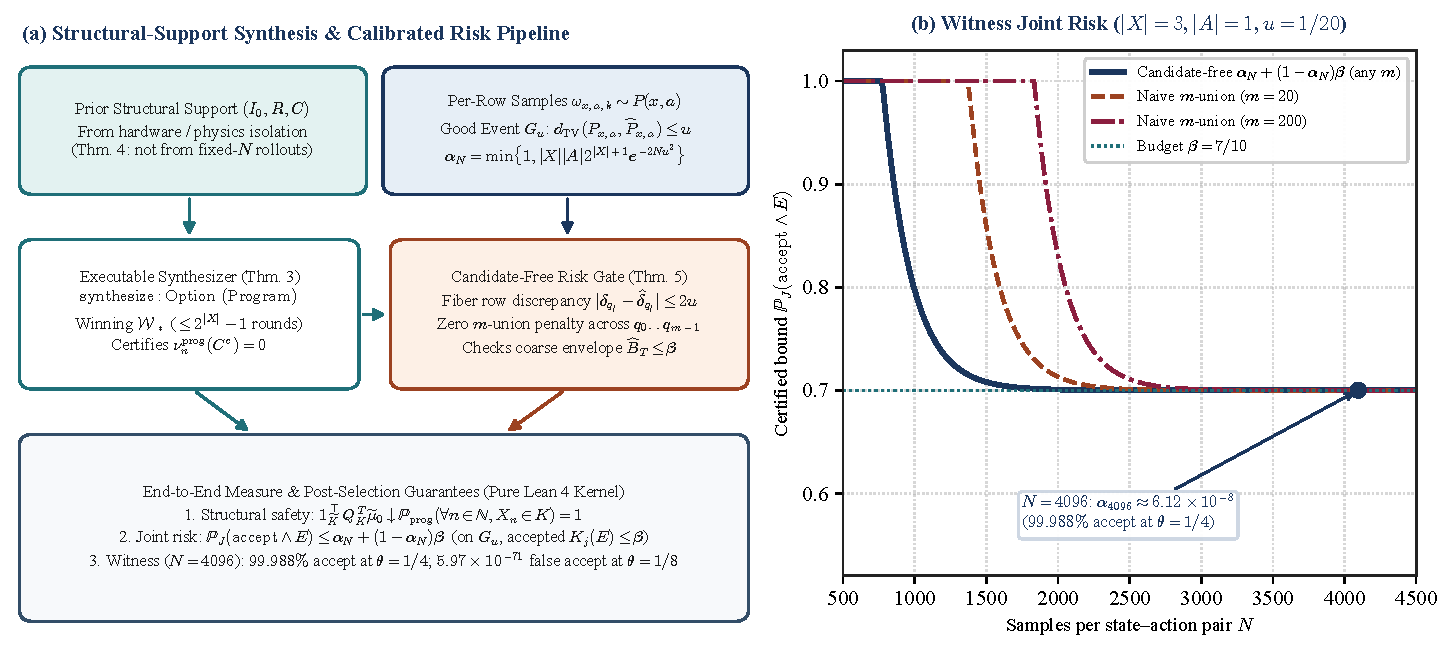
\includegraphics[width=0.99\linewidth,height=\textheight,keepaspectratio,alt={End-to-end
pure-kernel synthesis and calibrated post-selection risk operating
curve. (a) Separation between sample-free perpetual safety from prior
structural support (I\_0 = \textbackslash mathrm\{supp\}(p\_0), R =
\textbackslash mathrm\{supp\}(P), C) and finite-horizon risk calibration
on G\_u across q\_0,\textbackslash dots,q\_\{m-1\} (Theorem 5). (b)
Exact binomial acceptance curve \textbackslash
mathbb\{P\}\_\textbackslash theta(\textbackslash
mathrm\{selectedAccepts\}) across true progress rates \textbackslash
theta on the three-state witness, showing near-unit acceptance when risk
margin exceeds 2u (\textbackslash theta=1/4), conservative abstention
inside the 2u-margin band (\textbackslash theta=1/5), and shrinkage of
that band under u\_N \textbackslash propto N\^{}\{-1/2\} (N=16\{,\}384,
u=1/40 at identical \textbackslash alpha \textbackslash approx 6.12
\textbackslash times
10\^{}\{-8\}).}]{figures/fig1_synthesis_and_calibration.pdf}
\caption{End-to-end pure-kernel synthesis and calibrated post-selection
risk operating curve. (a) Separation between sample-free perpetual
safety from prior structural support
\((I_0 = \mathrm{supp}(p_0), R = \mathrm{supp}(P), C)\) and
finite-horizon risk calibration on \(G_u\) across \(q_0,\dots,q_{m-1}\)
(Theorem 5). (b) Exact binomial acceptance curve
\(\mathbb{P}_\theta(\mathrm{selectedAccepts})\) across true progress
rates \(\theta\) on the three-state witness, showing near-unit
acceptance when risk margin exceeds \(2u\) (\(\theta=1/4\)),
conservative abstention inside the \(2u\)-margin band (\(\theta=1/5\)),
and shrinkage of that band under \(u_N \propto N^{-1/2}\)
(\(N=16{,}384, u=1/40\) at identical
\(\alpha \approx 6.12 \times 10^{-8}\)).}
\end{figure}

\subsection{Evaluating non-trivial abstraction selection against
microscopic-reference
verification}\label{evaluating-non-trivial-abstraction-selection-against-microscopic-reference-verification}

The formalized three-state witness above tests the risk gate cleanly
(\texttt{\textbar{}A\textbar{}\ =\ 1}, with coarse \(q_0\) pooling start
and goal so every accepted run uses \(q_1 = \mathrm{id}\)), leaving open
a practical question: \emph{when multiple non-identity coarse
abstractions synthesize valid controllers, what concrete sensor, memory,
and verification savings does macro-reference selection buy relative to
evaluating the selected coarse controller directly on the empirical
microscopic model \(\widehat{P}(\omega)\)?} Note that on \(G_u\),
evaluating any fixed coarse controller \(\mathrm{prog}_j\) directly on
\(\widehat{P}(\omega)\) also requires no \(m\)-union bound and pays only
\(T u\) (avoiding both \(T\widehat{\delta}_{q_j}\) and coarse-envelope
slack), at the cost of summing microscopic state trajectories of
cardinality up to \(|X|^{T+1}\).

To quantify these trade-offs on common datasets,
\texttt{verify\_standalone.py} evaluates a \(12\)-state, \(3\)-action
(\texttt{boost}, \texttt{steady}, \texttt{hazard}), horizon-\(T=4\)
staged pipeline (\(K = \{0,\dots,10\}\), unsafe cemetery \(\bot = 11\),
uniform initial law \(p_0\) over \(S_A \cup S_B = \{0,\dots,7\}\),
target set \(G = G_{\mathrm{buf}} \cup G_{\mathrm{main}}\) with
\(G_{\mathrm{buf}} = \{8\}\) and \(G_{\mathrm{main}} = \{9,10\}\)). On
stage \(S_A = \{0,1,2,3\}\), \texttt{boost} is safe and reaches \(G\)
w.p. \(0.70\) (\(0.69\) on \(\{2,3\}\)); on delicate stage
\(S_B = \{4,5,6,7\}\) and quiet buffer goal
\(G_{\mathrm{buf}} = \{8\}\), \texttt{boost} leaks to \(\bot\) w.p.
\(1/2\) whereas \texttt{steady} is safe and reaches \(G\) w.p. \(0.60\)
(\(0.59\) on \(\{6,7,8\}\)). Compare four abstractions (Table 3):
\emph{(i)} \(q_{\mathrm{pool3}}\) (\(|Y|=3\): pools \(\{0,\dots,8\}\)),
which forces \texttt{steady} everywhere (true missed-\(G\) risk
\(0.07836\)) and has \(\delta_{q_{\mathrm{pool3}}} = 1\); \emph{(ii)}
non-identity \(q_{\mathrm{coarse4}}\) (\(|Y|=4\): separates \(S_A\) from
\(S_B \cup G_{\mathrm{buf}}\)), whose synthesized controller plays
\texttt{boost} on \(S_A\) and \texttt{steady} on
\(S_B \cup G_{\mathrm{buf}}\) (cutting true risk to \textbf{\(0.04469\)}
with \(\delta_{q_{\mathrm{coarse4}}} = 1/100\), while paying
\(+0.01069\) coarse-envelope slack from pooling \(G_{\mathrm{buf}}\)
with \(S_B\)); \emph{(iii)} non-identity \(q_{\mathrm{fine5}}\)
(\(|Y|=5\): isolates \(G_{\mathrm{buf}}\)), achieving true risk
\textbf{\(0.04469\)} with \textbf{only \(4\) reachable memory states}
(vs.~\(11\) under \(q_{\mathrm{id12}}\)) and zero envelope overshoot;
and \emph{(iv)} full-state / microscopic-reference evaluation on
\(\widehat{P}\) (\(|X|=12\)).

\Needspace{28\baselineskip}

{\def\LTcaptype{none} % do not increment counter
\begin{longtable}[]{@{}
  >{\raggedright\arraybackslash}p{(\linewidth - 10\tabcolsep) * \real{0.1667}}
  >{\raggedright\arraybackslash}p{(\linewidth - 10\tabcolsep) * \real{0.1667}}
  >{\raggedright\arraybackslash}p{(\linewidth - 10\tabcolsep) * \real{0.1667}}
  >{\raggedright\arraybackslash}p{(\linewidth - 10\tabcolsep) * \real{0.1667}}
  >{\raggedright\arraybackslash}p{(\linewidth - 10\tabcolsep) * \real{0.1667}}
  >{\raggedright\arraybackslash}p{(\linewidth - 10\tabcolsep) * \real{0.1667}}@{}}
\toprule\noalign{}
\begin{minipage}[b]{\linewidth}\raggedright
Abstraction / Verifier
\end{minipage} & \begin{minipage}[b]{\linewidth}\raggedright
Sensor \(\lvert Y\rvert\) \& Reach. Memory
\end{minipage} & \begin{minipage}[b]{\linewidth}\raggedright
True \(\delta_q\) \& True Risk \(K_j(E)\)
\end{minipage} & \begin{minipage}[b]{\linewidth}\raggedright
Pos. Ref. Paths \& Exact Eval Time
\end{minipage} & \begin{minipage}[b]{\linewidth}\raggedright
\(100\)-Trial Accept (\(\tau{=}0.125,\) \(\beta{=}0.34\))
\end{minipage} & \begin{minipage}[b]{\linewidth}\raggedright
Abstention Breakdown (Fiber / Env. / \(u{+}\widehat{\delta}\))
\end{minipage} \\
\midrule\noalign{}
\endhead
\bottomrule\noalign{}
\endlastfoot
\(q_{\mathrm{pool3}}\) (\texttt{steady} only) & \(\lvert Y\rvert=3\),
mem \(3\) & \(\delta=1\), risk \(0.07836\) & \(5\) paths
(\(0.5\text{ ms}\)) & \(0\%\) (rejected \(100\%\)) & Cleanly rejected
(\(\widehat{\delta}-2u > \tau\)) \\
\(q_{\mathrm{coarse4}}\) (non-id, menu A) & \(\lvert Y\rvert=4\), mem
\(5\) & \(\delta=\frac{1}{100}\), risk \(0.04469\) & \textbf{\(20\)
paths (\(0.9\text{ ms}\))} & \textbf{\(56\%\)} (\(96\%\) at
\(\beta{=}0.38\)) & \(0\%\) / \(15\%\) / \(29\%\) (\(51\%\) fiber,
\(\tau{=}0.095\)) \\
\(q_{\mathrm{fine5}}\) (non-id, menu B) & \(\lvert Y\rvert=5\),
\textbf{mem \(4\)} & \(\delta=\frac{1}{100}\), risk \(0.04469\) &
\textbf{\(62\) paths (\(1.7\text{ ms}\))} & \textbf{\(75\%\)} (\(99\%\)
at \(\beta{=}0.38\)) & \(0\%\) / \(0\%\) / \(25\%\) (\(41\%\) fiber,
\(\tau{=}0.095\)) \\
Micro-ref \(\widehat{P}\) / \(q_{\mathrm{id12}}\) &
\(\lvert X\rvert=12\), mem \(11\) & \(\delta=0\), risk \(0.04469\) &
\(8{,}248\) paths (\(135\text{ ms}\)) & \(100\%\) (even at
\(\beta{=}0.20\)) & Pays \(Tu=0.10\) only;
\textbf{\(72\times\)--\(147\times\) slower} \\
\end{longtable}
}

Table 3. Multi-abstraction comparison on the \(12\)-state, \(3\)-action,
\(T=4\) benchmark across \(100\) seeded datasets (\(N=2500\) per row,
\(u = 1/40\); reproduced by \texttt{verify\_standalone.py}).

Across \(100\) seeded training datasets (\(N=2500, u=1/40\)), Table 3
isolates three concrete design lessons: \emph{(i)} non-identity
abstractions \(q_{\mathrm{coarse4}}\) and \(q_{\mathrm{fine5}}\) reduce
controller memory (\(4\)--\(5\) states vs.~\(11\)), sensor cardinality
(\(4\)--\(5\) vs.~\(12\)), and exact rational reference-verification
paths from \(8{,}248\) to \(20\)--\(62\)
(\textbf{\(72\times\)--\(147\times\) faster} than microscopic
\(\widehat{P}\) evaluation) while matching optimal full-state risk
(\(0.04469\) vs.~\(0.07836\)); \emph{(ii)} candidate ordering matters
because \texttt{selectCandidate} commits to the first \(\tau\)-certified
index before checking \(\widehat{B}_T \le \beta\): at
\(\tau = 0.125, \beta = 0.34\), Menu A
(\([q_{\mathrm{pool3}}, q_{\mathrm{coarse4}}, q_{\mathrm{fine5}}]\))
abstains on \(19\%\) more runs than Menu B
(\([q_{\mathrm{pool3}}, q_{\mathrm{fine5}}, q_{\mathrm{coarse4}}]\):
\(56\%\) vs.~\(75\%\) acceptance, including \(15\%\) from
\(q_{\mathrm{coarse4}}\)'s coarse-envelope slack and \(25\%\)--\(29\%\)
from \((u+\widehat{\delta})\) margins), whereas tightening \(\tau\) to
\(0.095\) triggers \(41\%\)--\(51\%\) \texttt{ambiguous}
fiber-discrepancy abstentions (\texttt{selectCandidate\ =\ none}); and
\emph{(iii)} when microscopic \(\widehat{P}\) evaluation is
computationally affordable, certifying the \emph{coarse} controller
\texttt{prog\_fine5} via \(\widehat{P}\) combines compact \(4\)-state
runtime deployment with tighter \(Tu\)-only statistical margins
(accepting \(10/10\) runs even at \(\beta = 0.20\)).

\section{Binary-observation belief quotients on standard Borel
spaces}\label{binary-observation-belief-quotients-on-standard-borel-spaces}

Sections 2--4 tracked hidden states either combinatorially via finite
supports \(S_n \in \mathcal{A}_q\) or approximately via empirical fiber
row-discrepancies \(\widehat{\delta}_q\). In general partially observed
Markov control on Polish or standard Borel state spaces
\((X, \Sigma_X)\)
\citep{bertsekasShreve1978, hernandezLerma1996, kallenberg2021}, optimal
and predictive controllers instead maintain a continuous \emph{belief
state} \(b \in \mathcal{P}(X)\) in the Giry space of probability
measures on \(X\), equipped with the Giry \(\sigma\)-algebra
\(\Sigma_{\mathcal{P}(X)}\) generated by the evaluation maps
\(b \mapsto b(E)\) for \(E \in \Sigma_X\) \citep{astrom1965, giry1982}.
Given a Markov transition kernel \(P: X \times A \to \mathcal{P}(X)\)
(\texttt{ProbabilityTheory.Kernel} in Mathlib) and a measurable binary
observation map \(q: X \to \{0,1\}\) (with deterministic observation
kernel \(O((x,a), \cdot) = \delta_{q(x)}\)), each belief--action pair
\((b,a)\) induces a predicted state measure
\(\widehat{b}_a := \int_X P(x,a)\, db(x)\), a predicted observation
measure
\(\bar{o}_{b,a} := q_\# \widehat{b}_a \in \mathcal{P}(\{0,1\})\),
and---because \(X\) is a standard Borel space---a measurable regular
conditional probability kernel (\texttt{posteriorKernel}) yielding the
Bayesian posterior belief \(\mathrm{Post}(b,a,y) \in \mathcal{P}(X)\)
uniquely for \(\bar{o}_{b,a}\)-almost every \(y \in \{0,1\}\). Pushing
\(\bar{o}_{b,a}\) forward through \(y \mapsto \mathrm{Post}(b,a,y)\)
defines the measurable \emph{posterior-belief transition kernel}
\(\mathcal{K}_{\mathrm{bel}}: \mathcal{P}(X) \times A \to \mathcal{P}(\mathcal{P}(X))\).

When can the infinite-dimensional belief space \(\mathcal{P}(X)\) be
compressed without loss to the one-dimensional observable coordinate
\(c_q: \mathcal{P}(X) \to [0,1]\) defined by
\(c_q(b) := b(q^{-1}(\{1\}))\)? Assume \(q\) is surjective, witnessed by
explicit representatives \(x_0, x_1 \in X\) with \(q(x_0) = 0\) and
\(q(x_1) = 1\). Then \(c_q\) maps \(\mathcal{P}(X)\) surjectively onto
the compact convex interval \([0,1]\) with explicit measurable affine
section \(\sigma_{x_0, x_1}: [0,1] \to \mathcal{P}(X)\) given by
\(\sigma_{x_0, x_1}(u) := (1 - u)\delta_{x_0} + u \delta_{x_1}\),
satisfying \(c_q(\sigma_{x_0, x_1}(u)) = u\) for all \(u \in [0,1]\).
Define the \emph{closed-tests condition} (\texttt{ClosedTests}) on
\((P, q)\) by requiring one-step observable transition invariance across
\(q\)-fibers
\citep{burkeRosenblatt1958, kemenySnell1960, paigeTarjan1987, larsenSkou1991, givanDeanGreig2003}:
\[\begin{aligned}
\mathrm{ClosedTests}(P, q) :\iff \forall x, x' \in X,\ q(x) = q(x') \implies \\
\forall a \in A,\ P(x,a)\bigl(q^{-1}(\{1\})\bigr) = P(x',a)\bigl(q^{-1}(\{1\})\bigr).
\end{aligned}\] For any finite action--observation test word
\(w = [(a_1, y_1), \dots, (a_k, y_k)] \in (A \times \{0,1\})^*\), define
the multi-step test response \(F_w: X \to [0,1]\) recursively by
\(F_{[]}(x) := 1\) and
\(F_{(a,y)::w'}(x) := \int_{q^{-1}(\{y\})} F_{w'}(z)\, P(x,a)(dz)\),
with belief test expectation \(T_w(b) := \int_X F_w(x)\, db(x)\)
\citep{jaeger2000, littmanSuttonSingh2001}.

\textbf{Theorem 6 (Closed-test characterization of measurable Markov
belief quotients).} \emph{Let \((X, \Sigma_X)\) be a nonempty standard
Borel space, \((A, \Sigma_A)\) a measurable action space,
\(P: X \times A \to \mathcal{P}(X)\) a Markov kernel, and
\(q: X \to \{0,1\}\) a measurable map with \(q(x_0) = 0\) and
\(q(x_1) = 1\).}

\begin{enumerate}
\def\labelenumi{\arabic{enumi}.}
\tightlist
\item
  \textbf{Necessary and sufficient belief-kernel descent.}
  \emph{\(\mathrm{ClosedTests}(P, q)\) holds if and only if there exists
  a unique Markov quotient kernel
  \(\bar{K}: [0,1] \times A \to \mathcal{P}([0,1])\) intertwining
  \(\mathcal{K}_{\mathrm{bel}}\) across every input belief
  \(b \in \mathcal{P}(X)\) and action \(a \in A\):}
  \[(c_q)_\# \mathcal{K}_{\mathrm{bel}}(b, a) = \bar{K}\bigl(c_q(b), a\bigr).\]
  \emph{Moreover, \(\bar{K}\) is given explicitly by pulling
  \(\mathcal{K}_{\mathrm{bel}}\) back along the affine section
  \(\sigma_{x_0, x_1}\) and pushing forward by \(c_q\); conversely,
  existence of \textbf{any} kernel \(\bar{K}\) (even without assuming
  \(\bar{K}\) is Markov) satisfying
  \((c_q)_\# \mathcal{K}_{\mathrm{bel}}(b,a) = \bar{K}(c_q(b), a)\) for
  all point-mass beliefs \(b = \delta_x\) already forces
  \(\mathrm{ClosedTests}(P, q)\).}
\item
  \textbf{Multi-step predictive sufficiency vs.~hidden-state safety
  non-descent.} \emph{Whenever the closed-tests property holds for
  \((P, q)\), every multi-step test expectation \(T_w(b)\)
  (\(w \in (A \times \{0,1\})^*\)), every observation-measurable reward
  \(\int_X r(q(x))\, db(x) = (1 - c_q(b))r(0) + c_q(b)r(1)\), and
  observable-class probabilities factor solely through \(c_q(b)\).
  Nevertheless, on the four-state parity-noise system \(X = \{0,1\}^2\)
  with binary actions \(A = \{0,1\}\), \(q(x_1, x_2) = x_1\),
  Bernoulli\((1/4)\) noise \(N\), and update mapping \((x_1, x_2)\)
  under \((a, N)\) to \((x_1 \oplus (a \land N),\, x_2 \oplus N)\),
  \(\mathrm{ClosedTests}(P, q)\) holds and
  \(\delta_{(0,0)}, \delta_{(0,1)}\) induce identical expectations on
  \textbf{all} future action--observation words \(w\), yet no function
  of \(c_q(b)\) can represent the latent reward
  \(\int \mathbf{1}\{x_2 = 1\}\, db\) or the latent safety probability
  \(b(\{x_2 = 0\})\), and perturbing step updates to \((x_2, x_2)\) at
  \(a = 1\) and \((x_1, x_2)\) at \(a = 0\) destroys
  \(\mathrm{ClosedTests}\) and eliminates any Markov belief quotient
  factoring through \(c_q\).}
\end{enumerate}

Theorem 6 (proved in Appendix A.5) serves as a clean boundary theorem
showing that \emph{exact predictive sufficiency can erase hidden safety
invariants}. Note its exact geometric and measure-theoretic scope under
deterministic binary \(q: X \to \{0,1\}\): on positive-probability
branches \(\bar{o}_{b,a}(\{y\}) > 0\), the posterior reduces directly to
the normalized fiber restriction
\(\widehat{b}_a(\cdot \cap q^{-1}(\{y\})) / \widehat{b}_a(q^{-1}(\{y\}))\),
while standard Borel \((X, \Sigma_X)\) is the setting adopted by our
Mathlib \texttt{posteriorKernel} formalization to package all branches
into a single measurable Markov kernel \(\mathcal{K}_{\mathrm{bel}}\).
While the input coordinate \(c_q(b) \in [0,1]\) varies continuously
across prior beliefs \(b \in \mathcal{P}(X)\), upon receiving
\(y \in \{0,1\}\) the posterior concentrates on \(q^{-1}(\{y\})\) so
\(c_q(\mathrm{Post}(b,a,y)) = y \in \{0,1\}\) for
\(\bar{o}_{b,a}\)-a.e.~\(y\) (rendering the pushforward immune to
null-branch conventions). Under \texttt{ClosedTests}, \(\bar{K}(u, a)\)
is explicitly the Bernoulli kernel on \(\{0,1\} \subseteq [0,1]\) with
success parameter \((1-u)p_0(a) + u p_1(a)\), where
\(p_i(a) := P(x_i, a)(q^{-1}(\{1\}))\); yet even when \(\bar{K}\)
exists, compressing beliefs through \(c_q\) erases decoupled hazardous
coordinates \(x_2\) (whereas finer belief representations retaining
\(x_2\) remain valid).

\section{Prepaid resource constraints, fault-mechanism discrimination,
and minimax
regret}\label{prepaid-resource-constraints-fault-mechanism-discrimination-and-minimax-regret}

\subsection{Serial versus correlated fault propagation under strict
prepayment}\label{serial-versus-correlated-fault-propagation-under-strict-prepayment}

In Sections 2--5, state uncertainty arose from coarse sensors while the
underlying transition mechanism \(P\) was fixed. In fault-tolerant
distributed stores, redundant avionics, and replicating register
assemblies \citep{athreyaNey1972, altman1999, cassandrasLafortune2021},
a second, deeper structural ambiguity arises: \textbf{how do faults
propagate across redundant components when active repair requires
prepaid operational budget?} If an action creates a healthy backup slot
and a subsequent step suffers a fault, does that fault corrupt only the
currently dispatched slot, or does a shared environmental shock
simultaneously corrupt the undispatched backup?

To analyze this question with complete mathematical transparency,
consider a dynamic register store initialized at step \(t = 0\) with a
single damaged root slot (\texttt{root0} holding bit \(\neg g\), where
\(g \in \{\mathrm{false}, \mathrm{true}\}\) is the public target bit)
and an initially absent secondary backup slot (\texttt{child1}
\(= \mathrm{none}\)). At each step \(t \in \{0, \dots, H-1\}\), nature
draws an independent tick mode
\(M_t \in \{\mathrm{normal}, \mathrm{fault}\}\) with
\(\mathbb{P}(M_t = \mathrm{normal}) = r \in [0,1] \cap \mathbb{Q}\) and
\(\mathbb{P}(M_t = \mathrm{fault}) = 1 - r\) (together with an
independent fair birth label retained in world lineage records). Two
candidate environmental fault mechanisms \(m \in \{S, G\}\) govern how
faults affect the store, with \(m\) fixed before \(t=0\) for the entire
run:

\begin{itemize}
\tightlist
\item
  \textbf{Serial local fault (\(S\)).} A normal step executes the
  requested operation on the addressed slot: idling a healthy slot
  (\texttt{bit} \(= g\)) or writing \(g\) to an existing slot produces
  one newborn (filling \texttt{child1} with a healthy bit \(g\) if
  \texttt{child1} was \texttt{none}, and appending subsequent births to
  tail records), whereas writing \(\neg g\) overwrites the addressed
  slot with \(\neg g\) and produces zero births. A fault step on an
  existing addressed slot corrupts \emph{only that addressed slot} to
  \(\neg g\), leaves undispatched slots intact, charges zero write fee,
  and produces zero births.
\item
  \textbf{Global correlated fault (\(G\)).} Normal-mode execution is
  identical to \(S\). Whenever a tick enters fault mode
  (\(M_t = \mathrm{fault}\)), however---including during idle requests,
  requests to an absent \texttt{child1}, or post-\texttt{stop}
  ticks---\emph{every currently living slot in the store} has its
  physical bit reset to \(\neg g\).
\end{itemize}

At each step, the controller selects from a seven-action menu
\(\mathcal{A}_7\): permanent \texttt{stop} (which commits the current
and all remaining steps to idling \texttt{root0} while world noise
continues), \texttt{idle} at \texttt{root0} or \texttt{child1},
\texttt{write\ false} at \texttt{root0} or \texttt{child1}, or
\texttt{write\ true} at \texttt{root0} or \texttt{child1}. Crucially,
the controller operates under \textbf{two strict physical constraints}:

\begin{enumerate}
\def\labelenumi{\arabic{enumi}.}
\tightlist
\item
  \textbf{Prepaid non-replenished wallet (\(B\)).} The controller begins
  with rational budget \(B_0 = B \ge 0\) and write tariff \(c > 0\).
  Every write request (\texttt{cap}\((a) = 1\); \texttt{stop} and
  \texttt{idle} have \texttt{cap}\((a) = 0\)) is filtered \emph{before}
  execution by the hard prepayment gate
  \(c \cdot \mathrm{cap}(a_t) \le B_t\). One cannot submit an
  unaffordable write hoping that a fault or absent slot will waive the
  actual charge. Only a normal-mode write to an existing slot deducts
  \(C_t = c\) (\(B_{t+1} = B_t - c\)); faulted writes, absent-slot
  writes, and idles deduct \(C_t = 0\).
\item
  \textbf{Two-bit transaction receipts.} After each step, the controller
  observes \emph{only} the two-bit receipt
  \(o_t = (\mathrm{birth}_t, \mathrm{paid}_t) \in \{0,1\}^2\), recording
  whether a birth occurred and whether tariff \(c\) was actually
  charged, without direct read access to internal slot bits, fault
  modes, or which mechanism \(m \in \{S, G\}\) is active.
\end{enumerate}

Notice immediately how \(S\) and \(G\) break naive state observers.
Suppose \(B \ge c\) and \(0 < r < 1\). At \(t=0\), the controller writes
\(g\) to \texttt{root0} and observes \(o_0 = (1, 1)\) (occurring w.p.
\(r\) under both \(S\) and \(G\)): \texttt{root0} is now repaired to
\(g\), \texttt{child1} is allocated with healthy bit \(g\), and
remaining wallet is \(B - c\). At \(t=1\), the controller idles
\texttt{root0} and observes \(o_1 = (0, 0)\) (occurring w.p. \(1-r\)
under both \(S\) and \(G\)). After this identical positive-probability
receipt prefix \([(1,1), (0,0)]\) (mass \(r(1-r)\)), the hidden store
under \(S\) has \((\mathrm{root0} = \neg g,\ \mathrm{child1} = g)\)---so
\texttt{child1} survives as an intact backup!---whereas under \(G\) the
fault wiped \emph{both} slots to
\((\mathrm{root0} = \neg g,\ \mathrm{child1} = \neg g)\). Under a prior
\(w = (w_S, w_G)\) over \(\{S, G\}\), the marginal posterior on \(m\)
after \([(1,1), (0,0)]\) is still \((w_S, w_G)\), yet \textbf{mechanism
identity and physical backup state have become strictly entangled}:
multiplying the mechanism marginal by the state marginal would fabricate
impossible worlds.

\subsection{Exact discrimination bounds, Bayes--minimax duality, and
strict benefit of
randomization}\label{exact-discrimination-bounds-bayesminimax-duality-and-strict-benefit-of-randomization}

Fix horizon \(H\), budget \(B\), tariff \(c > 0\), fee price
\(\lambda \ge 0\), and discount \(d \in [0,1]\), evaluating any causal
policy \(\pi\) (permitted to use complete action--receipt histories plus
arbitrary real-valued private randomness independent of \(m\) and world
noise) under mechanism \(m \in \{S, G\}\) by net discounted payoff
\[J_m(\pi) := \mathbb{E}_m^\pi\!\left[\sum_{t=0}^{H-1} d^t \bigl(\mathrm{birth}_t - \lambda C_t\bigr)\right].\]
Let \(P_m^\pi\) denote the induced probability distribution over
complete length-\(H\) action--receipt histories (and private-seed
decision tables), and let
\(\Delta_{H,B} := \sup_\pi d_{\mathrm{TV}}(P_S^\pi, P_G^\pi)\) be the
maximum total-variation distinguishability achievable by \emph{any}
legal adaptive experiment
\citep{blackwell1953, leCam1973, coverThomas2006}. Simultaneously, let
\(V_m^* := \sup_\pi J_m(\pi)\) denote the oracle optimal value when
\(m\) is known (subject to the same receipt interface and wallet \(B\)),
and define \emph{worst-case minimax regret} \citep{wald1950, savage1951}
across unknown \(m \in \{S, G\}\) by
\[R_m(\pi) := V_m^* - J_m(\pi), \qquad R(\pi) := \max_{m \in \{S, G\}} R_m(\pi), \qquad R^* := \inf_\pi R(\pi).\]
Notice that for any prior weights
\(w = (w_S, w_G) \in \Delta(\{S, G\})\), if
\(V_w^* := \sup_\pi (w_S J_S(\pi) + w_G J_G(\pi))\) is the Bayes-optimal
value on the joint \texttt{(mechanism,\ store)} belief state
\citep{bellman1957, blackwell1965, smallwoodSondik1973}, then every
legal policy \(\pi\) satisfies
\(R(\pi) \ge w_S R_S(\pi) + w_G R_G(\pi) \ge w_S V_S^* + w_G V_G^* - V_w^*\).
Thus, exhibiting a dual weight vector \(w\) and a concrete legal policy
\(\rho\) satisfying the sandwich identity
\[L(w) := w_S V_S^* + w_G V_G^* - V_w^* = \max_{m \in \{S,G\}} \bigl(V_m^* - J_m(\rho)\bigr) =: U(\rho)\]
certifies \emph{both} the exact minimax regret \(R^* = L(w) = U(\rho)\)
over all full-history real-randomized behavioral and private-seed
policies (\texttt{RawCausalPolicy}) \emph{and} optimality of \(\rho\)
\citep{vonNeumann1928}.

\Needspace{28\baselineskip}

{\def\LTcaptype{none} % do not increment counter
\begin{longtable}[]{@{}
  >{\raggedright\arraybackslash}p{(\linewidth - 10\tabcolsep) * \real{0.1667}}
  >{\raggedleft\arraybackslash}p{(\linewidth - 10\tabcolsep) * \real{0.1667}}
  >{\raggedleft\arraybackslash}p{(\linewidth - 10\tabcolsep) * \real{0.1667}}
  >{\raggedleft\arraybackslash}p{(\linewidth - 10\tabcolsep) * \real{0.1667}}
  >{\raggedleft\arraybackslash}p{(\linewidth - 10\tabcolsep) * \real{0.1667}}
  >{\raggedleft\arraybackslash}p{(\linewidth - 10\tabcolsep) * \real{0.1667}}@{}}
\toprule\noalign{}
\begin{minipage}[b]{\linewidth}\raggedright
Policy / Quantity
\end{minipage} & \begin{minipage}[b]{\linewidth}\raggedleft
Payoff \(J_S(\cdot)\) under \(S\)
\end{minipage} & \begin{minipage}[b]{\linewidth}\raggedleft
Payoff \(J_G(\cdot)\) under \(G\)
\end{minipage} & \begin{minipage}[b]{\linewidth}\raggedleft
Regret \(R_S(\cdot)\)
\end{minipage} & \begin{minipage}[b]{\linewidth}\raggedleft
Regret \(R_G(\cdot)\)
\end{minipage} & \begin{minipage}[b]{\linewidth}\raggedleft
Max Regret \(R(\cdot)\)
\end{minipage} \\
\midrule\noalign{}
\endhead
\bottomrule\noalign{}
\endlastfoot
Oracle \(S\)-table \(\pi_S\) & \(41/32\) & \(37/32\) & \(0\) & \(3/32\)
& \(3/32 = 12/128\) \\
Oracle \(G\)-table \(\pi_G\) (best det.) & \(40/32\) & \(40/32\) &
\(1/32\) & \(0\) & \(1/32 = 4/128\) \\
Seeded mixture \(\rho = \frac{1}{4}\pi_S + \frac{3}{4}\pi_G\) &
\(161/128\) & \(157/128\) & \(3/128\) & \(3/128\) & \textbf{\(3/128\)}
(\(= R^*\)) \\
\end{longtable}
}

Table 4. Exact three-step payoff and regret matrix at
\((r, H, B, c, \lambda, d) = (1/2, 3, 2, 1, 1/4, 1)\), verified purely
inside the Lean 4 kernel (\texttt{kernel\_int\_h3}). Dual weights
\(w = (3/4, 1/4)\) give \(V_w^* = 5/4 = 40/32\) and
\(L(w) = \frac{3}{4}\cdot\frac{41}{32} + \frac{1}{4}\cdot\frac{40}{32} - \frac{5}{4} = \frac{3}{128}\).

\textbf{Theorem 7 (Exact fault-discrimination bound, minimax regret
duality, and deterministic lattice gap).} \emph{Consider the prepaid
register fault model with mechanisms \(\{S, G\}\) starting from a single
damaged root.}

\begin{enumerate}
\def\labelenumi{\arabic{enumi}.}
\tightlist
\item
  \textbf{Exact path-coupling distinguishability.} \emph{Across all
  real-randomized adaptive history strategies (including shared private
  randomness between controller and terminal classifier),
  \(\Delta_{H,B} = 0\) whenever \(H \le 2\), whenever \(B < c\),
  whenever \(r \in \{0,1\}\), or whenever only \texttt{root0} is
  dispatched. At horizon \(H = 3\),}
  \[\Delta_{3,B} = \begin{cases} r^2(1 - r), & B \ge c, \\ 0, & B < c, \end{cases}\]
  \emph{attained when \(B \ge c\) by the three-step probe
  \texttt{write\ g\ to\ root0} \(\to\) \texttt{idle\ root0} \(\to\)
  \texttt{idle\ child1}, whose receipt trace \([(1,1), (0,0), (1,0)]\)
  has probability \(r^2(1-r)\) under \(S\) and \(0\) under \(G\).
  Moreover, for every \(H \ge 1\) and \(r \in (0,1)\), shared all-fault
  mass \((1-r)^H\) forces every total binary classifier under equal
  priors to incur error at least \((1-r)^H / 2 > 0\) (and at
  \(H=3, r=1/2\), minimum classification error is
  \(\frac{1}{2}(1 - 1/8) = 7/16\)). Nevertheless, observational
  indistinguishability need not force decision loss: at
  \((r, H, B, c, \lambda, d) = (1/2, 2, 2, 1, 1/4, 1)\),
  \(\Delta_{2,2} = 0\) yet a single deterministic table attains
  \(V_S^* = V_G^* = 13/16\) simultaneously.}
\item
  \textbf{Exact minimax regret and strict randomization advantage.}
  \emph{Fix \((r, H, B, c, \lambda, d) = (1/2, 3, 2, 1, 1/4, 1)\) with
  \(g = \mathrm{true}\). Then:}

  \begin{itemize}
  \tightlist
  \item
    \emph{The full-menu oracle values are \(V_S^* = 41/32\) and
    \(V_G^* = 40/32 = 5/4\), with cross-evaluations
    \(J_G(\pi_S) = 37/32\) and \(J_S(\pi_G) = 40/32\);}
  \item
    \emph{Under dual weights \(w = (3/4, 1/4)\), the joint-belief Bayes
    value is \(V_w^* = 5/4\), yielding \(L(w) = 3/128\);}
  \item
    \emph{Drawing an independent uniform four-point private seed
    \(u \in \{0,1,2,3\}\) at initialization to execute \(\pi_S\) if
    \(u = 0\) and \(\pi_G\) if \(u \in \{1,2,3\}\) satisfies every
    prefix prepayment constraint \(B_t = 2 - \sum_{j<t} C_j \ge 0\)
    pathwise and achieves \(J_S(\rho) = 161/128\) and
    \(J_G(\rho) = 157/128\), establishing \(R^* = R(\rho) = 3/128\) over
    all real-randomized history strategies;}
  \item
    \emph{Every deterministic permitted-history strategy
    \(\pi_{\mathrm{det}}\) satisfies
    \(J_m(\pi_{\mathrm{det}}) \in \frac{1}{32}\mathbb{Z}\), forcing
    \(R(\pi_{\mathrm{det}}) \ge 1/32 > 3/128\) (with \(1/32\) attained
    by \(\pi_G\)).}
  \end{itemize}
\end{enumerate}

Theorem 7 (proved in Appendix A.6) illuminates the precise interplay
between information, budget, and randomization (Figure 2). Why do
\(\pi_S\) and \(\pi_G\) diverge at the third step? Only along the
ambiguous prefix \([(1,1), (0,0)]\) (probability \(1/4\), remaining
wallet \(1\), one step left): under \(S\), idling \texttt{child1} is
free and yields conditional expected payoff \(1/2\), beating a paid
re-write of \texttt{root0} (\(1/2 - 1/4 \cdot 1/2 = 3/8\)); under \(G\),
\texttt{child1} was wiped by the correlated fault, so idling
\texttt{child1} yields \(0\) while re-writing \texttt{root0} yields
\(3/8\). Note also two sharp conceptual distinctions: first, the dual
weights \(w = (3/4, 1/4)\) certifying the minimax lower bound are
\emph{opposite} to the deployment mixture weights \((1/4, 3/4)\) in
\(\rho\); second, although \(H=3\) is the earliest horizon at which an
experiment can distinguish \(S\) from \(G\) (\(\Delta_{3,2} = 1/8\)),
the distinguishing receipt arrives at the \emph{terminal} tick \(t=2\),
too late to inform earlier actions within that three-step task---which
is precisely why hedging via pre-committed private randomness reduces
worst-case regret from \(4/128\) to \(3/128\).

\begin{figure}
\centering
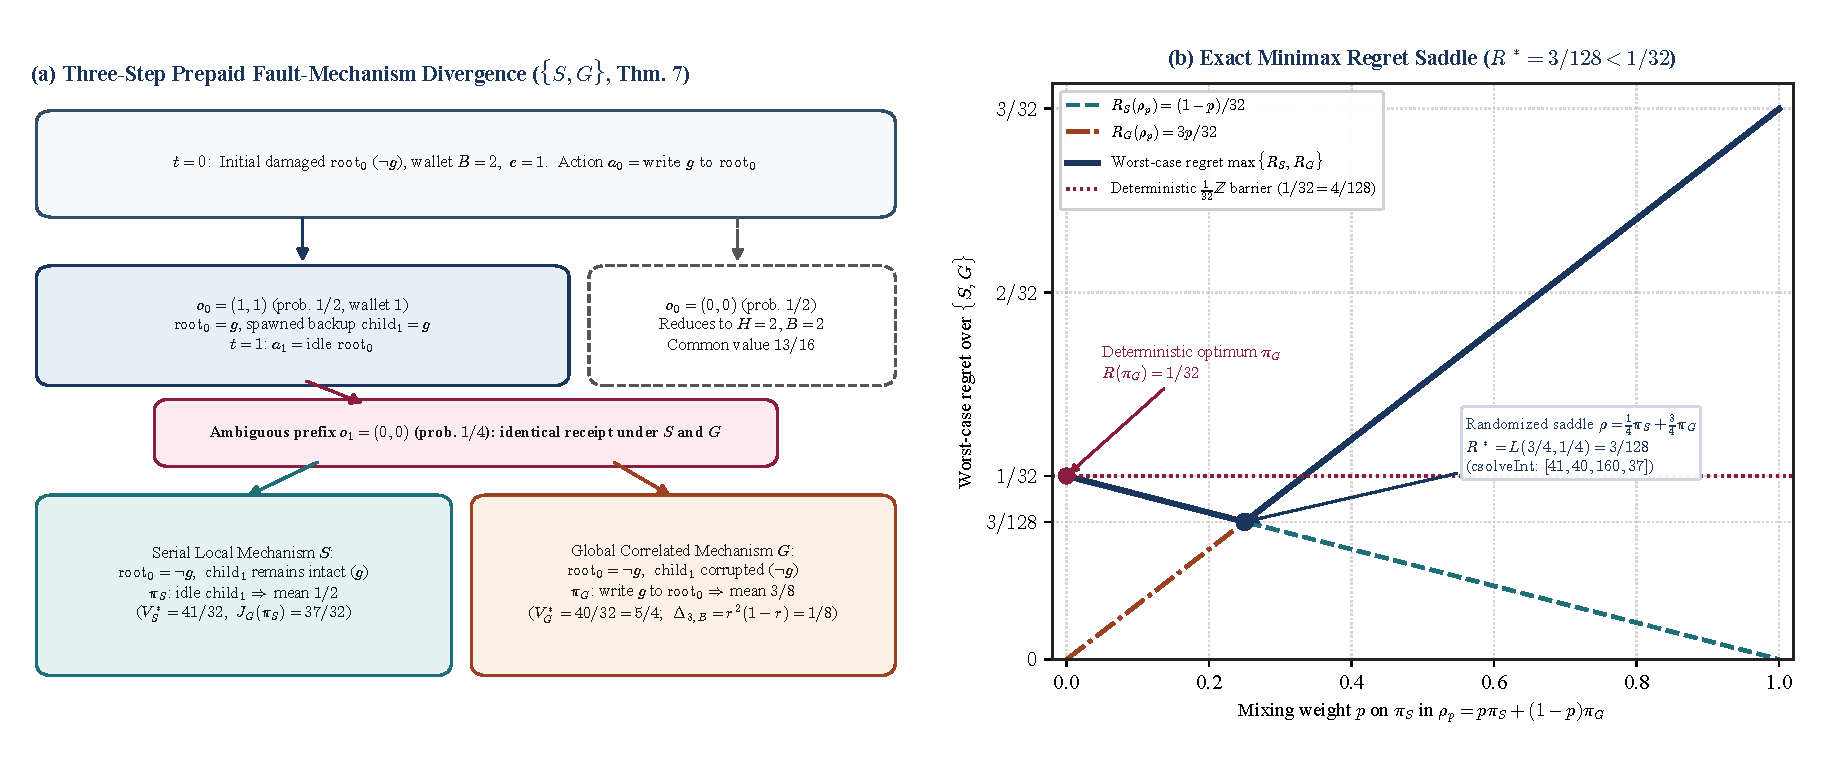
\includegraphics[width=0.99\linewidth,height=\textheight,keepaspectratio,alt={Three-step
prepaid fault-mechanism divergence and exact minimax regret saddle
(Theorem 7). (a) Branching register trajectory along the ambiguous
prefix o\_0=(1,1), o\_1=(0,0) separating serial local faults (S,
\textbackslash mathrm\{child\}\_1 intact) from global correlated faults
(G, \textbackslash mathrm\{child\}\_1 wiped) with exact total-variation
gap \textbackslash Delta\_\{3,B\} = r\^{}2(1-r) = 1/8. (b) Worst-case
regret envelope \textbackslash max\textbackslash\{R\_S(\textbackslash
rho\_p), R\_G(\textbackslash rho\_p)\textbackslash\} over mixtures
\textbackslash rho\_p = p\textbackslash pi\_S + (1-p)\textbackslash
pi\_G, showing the deterministic \textbackslash
frac\{1\}\{32\}\textbackslash mathbb\{Z\} lattice barrier (1/32 = 4/128
at \textbackslash pi\_G) and the exact randomized minimax saddle R\^{}*
= 3/128 at p = 1/4 certified inside the Lean 4 kernel via
csolveInt.}]{figures/fig2_fault_regret_and_kernel_dp.pdf}
\caption{Three-step prepaid fault-mechanism divergence and exact minimax
regret saddle (Theorem 7). (a) Branching register trajectory along the
ambiguous prefix \(o_0=(1,1), o_1=(0,0)\) separating serial local faults
(\(S\), \(\mathrm{child}_1\) intact) from global correlated faults
(\(G\), \(\mathrm{child}_1\) wiped) with exact total-variation gap
\(\Delta_{3,B} = r^2(1-r) = 1/8\). (b) Worst-case regret envelope
\(\max\{R_S(\rho_p), R_G(\rho_p)\}\) over mixtures
\(\rho_p = p\pi_S + (1-p)\pi_G\), showing the deterministic
\(\frac{1}{32}\mathbb{Z}\) lattice barrier (\(1/32 = 4/128\) at
\(\pi_G\)) and the exact randomized minimax saddle \(R^* = 3/128\) at
\(p = 1/4\) certified inside the Lean 4 kernel via
\protect\texttt{csolveInt}.}
\end{figure}

\section{Pure-kernel Lean 4 formalization architecture, GCD-free integer
reduction, and related
work}\label{pure-kernel-lean-4-formalization-architecture-gcd-free-integer-reduction-and-related-work}

\subsection{Decoupling executable synthesis and rational oracles from
classical measure
semantics}\label{decoupling-executable-synthesis-and-rational-oracles-from-classical-measure-semantics}

A recurring architectural tension in formalizing stochastic control
inside dependent type theory
\citep{mouraUllrich2021, mathlib2020, carneiro2019} is that realistic
theorems must speak about standard mathematical objects---Lebesgue
integrals, regular conditional probabilities on standard Borel spaces,
Kolmogorov infinite-trajectory extensions, and real exponential
Hoeffding bounds---all of which in Mathlib are \texttt{noncomputable}
and rely on \texttt{Classical.choice}, whereas synthesized controllers
and statistical acceptance gates must be \emph{genuinely executable
programs} free of classical axioms at runtime.

Our Lean 4 architecture resolves this tension through a strict
\textbf{two-layer semantic bridge}:

\begin{enumerate}
\def\labelenumi{\arabic{enumi}.}
\tightlist
\item
  \textbf{Purely computable syntax and decision layer.} In
  \texttt{ExecutableSupportController}, the controller type
  \texttt{Program\ X\ Y\ A} stores
  \texttt{initialMemory\ :\ Y\ →\ Finset\ X},
  \texttt{action\ :\ Finset\ X\ →\ A}, and
  \texttt{update\ :\ Finset\ X\ →\ A\ →\ Y\ →\ Finset\ X}. The
  synthesizer \texttt{synthesize} uses \texttt{Finset.filter},
  \texttt{List.find?}, and bounded Boolean recursion up to
  \(2^{|X|} - 1\). Likewise, in \texttt{NoisyFiniteRiskOracle},
  empirical masses, \(L_1\)/TV overlaps
  \(1 - \sum_z \min\{\widehat{p}(z), \widehat{p}'(z)\}\), fiber defects
  \(\widehat{\delta}_q\), three-valued interval decisions
  (\texttt{certified}, \texttt{rejected}, \texttt{ambiguous}),
  representative selection (\texttt{Finset.min\textquotesingle{}} under
  an explicit \texttt{LinearOrder\ X}), reference history sums, and
  \texttt{selectedAccepts} are written entirely over computable Lean
  types (\texttt{Nat}, \texttt{Rat}, \texttt{Bool}, and
  \texttt{Option}). None of these definitions imports \texttt{PMF} or
  \texttt{Measure}.
\item
  \textbf{Noncomputable measure-theoretic interpretation layer.} Only in
  proof sections do we lift a \texttt{Program} via \texttt{PMF.pure} to
  a stochastic \texttt{FiniteMemoryController}, embed empirical count
  ratios into \texttt{PMF.toMeasure}, construct the Ionescu--Tulcea
  trajectory measure \texttt{stateTrajMeasure} on
  \((X \times \mathrm{Finset}\ X)^{\mathbb{N}}\), and apply Hoeffding
  concentration on the product row law (\texttt{productRowLaw} in
  \texttt{VariableRegisteredSamples}). Bridge lemmas
  (\texttt{empiricalTV\_eq}, \texttt{referenceRisk\_eq}, and
  \texttt{memory\_eq\_traceSupport}) prove exact equality between the
  rational/combinatorial runtime outputs and their measure-theoretic
  counterparts, transferring \texttt{accepts\ =\ true} directly into
  real probability bounds without ever requiring runtime code to compute
  with reals.
\end{enumerate}

\subsection{\texorpdfstring{Eliminating \texttt{native\_decide} via
GCD-free integer-scaled dynamic
programming}{Eliminating native\_decide via GCD-free integer-scaled dynamic programming}}\label{eliminating-native_decide-via-gcd-free-integer-scaled-dynamic-programming}

The most instructive formal-verification obstacle in this work arose in
certifying \texttt{exact\_cached\_data} and \texttt{exact\_two\_data}
for Theorem 7 (\texttt{RegisterMechanismDecisionConsumer}). Evaluating
the exact Bayes-optimal value \(V_3^*(b_0, 2)\) over the joint
\texttt{(FaultMechanism\ ×\ Store)} belief space explores all \(7\)
actions and \(4\) two-bit receipts across depth \(3\) (\(28\)
action--observation branches per node). In the general rational POMDP
solver (\texttt{FiniteJointDecisionSolver}), every positive-mass receipt
\((a, o)\) updates the rational belief \(b \in \Delta(\mathcal{W})\) via
normalized Bayes division:
\[b^{a,o}(w') = \frac{\sum_{w,z} b(w)\, P(z \mid w)\, \mathbf{1}\{O(w,a,z)=o,\ T(w,a,z)=w'\}}{m_b^a(o)} \in \mathbb{Q}.\]
In Lean 4, each rational addition and division (\texttt{ℚ}) maintains
coprime numerator/denominator normal form by invoking \texttt{Nat.gcd}.
Inside compiled native code (\texttt{\#eval} or
\texttt{native\_decide}), Euclidean GCD over small integers runs
quickly. Inside Lean's \textbf{logical kernel reducer}
(\texttt{decide}), however, unfolding nested \texttt{Nat.gcd} recursion
across hundreds of rational belief-normalization nodes triggers severe
term blowup. A common shortcut in both Coq (\texttt{native\_compute};
\citet{boespflug2011}) and Lean 4 (\texttt{native\_decide}) delegates
Boolean evaluation to compiled code, introducing the compiler-trust
axiom \texttt{Lean.ofReduceBool} (\texttt{Lean.trustCompiler}). Keeping
proof terms verified without \texttt{Lean.ofReduceBool} cleanly
separates \emph{kernel proof-term verification} from trusting
compiled-binary execution \citep{mouraUllrich2021, carneiro2019}.

To verify Theorem 7's full-menu dynamic-programming certificates inside
Lean's kernel with zero compiler-trust axioms, we designed an exact
\emph{unnormalized integer-scaled dynamic programming mirror}
(\texttt{csolveInt} and \texttt{csourceInt}) and proved its bisimulation
with the rational Bayes solver (\texttt{csolveInt\_spec}):

\begin{enumerate}
\def\labelenumi{\arabic{enumi}.}
\tightlist
\item
  \textbf{Unnormalized integer beliefs (\texttt{UBelief}).} Represent an
  unnormalized belief as an association list
  \(U = [(w_1, u_1), \dots, (w_k, u_k)]\) with positive integer weights
  (\texttt{List\ (World\ ×\ Nat)}), total weight
  \(\mathrm{usum}(U) := \sum_i u_i \in \mathbb{N}\), and linear
  functional \(\mathrm{uexpect}(U, f) := \sum_i u_i f(w_i)\). Define the
  representation invariant \texttt{Represents}\((U, b)\) by
  \[\mathrm{usum}(U) > 0 \quad \land \quad \forall f: \mathcal{W} \to \mathbb{Q},\ \mathrm{uexpect}(U, f) = \mathrm{usum}(U) \cdot \mathbb{E}_b[f].\]
  At \(r = 1/2\), clearing the \(1/2\) tick-mode denominator updates
  \(U \mapsto U'_{a,o} := \mathrm{unext}(U, a, o)\) purely by integer
  list insertion (\texttt{uinsert}), satisfying the division-free
  identity \(2\,\mathrm{usum}(U)\, m_b^a(o) = \mathrm{usum}(U'_{a,o})\)
  and preserving \texttt{Represents}\((U'_{a,o}, b^{a,o})\) whenever
  \(\mathrm{usum}(U'_{a,o}) > 0\).
\item
  \textbf{Dyadic horizon-and-tariff scaling.} At price
  \(\lambda = 1/4\),
  \(4 \cdot \mathrm{gain}(a,o) = \mathrm{gain}_4(o) := 4\,\mathbf{1}\{\mathrm{birth}\} - \mathbf{1}\{\mathrm{paid}\} \in \mathbb{Z}\).
  Defining the integer dynamic program
  \texttt{csolveInt}\((n, (U, \mathrm{bal})) \in \mathbb{Z} \times \mathrm{CTree}_n\)
  recursively at remaining horizon \(n+1\) by summing over
  \(o \in \{0,1\}^2\) the branch score
  \[\mathrm{stepObs}(o) := \begin{cases}
  0, & \mathrm{usum}(U'_{a,o}) = 0, \\
  2^n \cdot \mathrm{usum}(U'_{a,o}) \cdot \mathrm{gain}_4(o) + \mathrm{csolveInt}_n(U'_{a,o}, \mathrm{bal}'_o)_1, & \mathrm{usum}(U'_{a,o}) > 0,
  \end{cases}\] and maximizing
  \(\sum_{o \in \{0,1\}^2} \mathrm{stepObs}(o)\) across legal actions
  \(a \in \mathrm{menuNat}(\mathrm{bal})\), satisfies---by induction on
  \(n\) with \emph{zero rational division}---the exact scaling invariant
  \[\bigl(\mathrm{csolveInt}_n(U, \mathrm{bal})_1 : \mathbb{Q}\bigr) = 4 \cdot 2^n \cdot \mathrm{usum}(U) \cdot V_n^*(b, \mathrm{bal}),\]
  together with exact equality of returned policy trees
  (\texttt{toTable\ =\ solve}) because positive scaling by
  \(c_{n+1} := 4 \cdot 2^{n+1} \cdot \mathrm{usum}(U) > 0\) preserves
  strict action inequalities
  (\(\mathrm{score}_{\mathbb{Z}}(a_1) < \mathrm{score}_{\mathbb{Z}}(a_2) \iff Q(a_1) < Q(a_2)\))
  and tie-breaking order (\texttt{cselectScored\_map}).
\item
  \textbf{Pure-kernel \texttt{decide} certification and measured
  verification profile.} Initializing
  \(U_{\mathrm{knownS}} = [(w_S, 1)]\) (\(\mathrm{usum} = 1\), scale
  \(4 \cdot 2^3 \cdot 1 = 32\)), \(U_{\mathrm{knownG}} = [(w_G, 1)]\)
  (scale \(32\)), and \(U_{\mathrm{dual}} = [(w_S, 3), (w_G, 1)]\)
  (\(\mathrm{usum} = 4\), scale \(4 \cdot 2^3 \cdot 4 = 128\)), Lean's
  kernel \texttt{decide} checks the seven integer equalities
  \[\mathrm{csolveInt}_3(U_S, 2)_1 = 41,\quad \mathrm{csolveInt}_3(U_G, 2)_1 = 40,\quad \mathrm{csolveInt}_3(U_{\mathrm{dual}}, 2)_1 = 160,\]
  \[\begin{aligned}
  \mathrm{csourceInt}(\pi_S, w_S) &= 41, \qquad \mathrm{csourceInt}(\pi_S, w_G) = 37, \\
  \mathrm{csourceInt}(\pi_G, w_S) &= 40, \qquad \mathrm{csourceInt}(\pi_G, w_G) = 40
  \end{aligned}\] in \texttt{Nat}/\texttt{Int} ring arithmetic, yielding
  \(41/32\), \(40/32 = 5/4\), \(160/128 = 5/4\), and \(37/32\) (and
  \(13 / (4 \cdot 2^2) = 13/16\) at \(H=2\) via
  \texttt{kernel\_int\_h2}). On the exact same \(H=3\), \(7\)-action,
  \(4\)-receipt belief-tree task
  (\texttt{\textbar{}FaultMechanism\ ×\ Store\textbar{}\ =\ 2\ ×\ 9\ =\ 18}
  reachable joint configurations), invoking \texttt{decide} directly on
  the rational \texttt{ℚ} solver (\texttt{cachedResult}) gets stuck on
  \texttt{Rat.inv} and \texttt{Belief}-subtype proof terms in the
  elaborator, and \texttt{decide\ +kernel} even at
  \texttt{maxHeartbeats\ =\ 12,000,000} (\texttt{maxRecDepth\ =\ 4096})
  times out in kernel fraction normalization; by contrast, our GCD-free
  integer mirror \texttt{RegisterMechanismDecisionConsumer} passes
  \texttt{decide} at default \texttt{maxHeartbeats\ =\ 200,000} and
  typechecks the entire module in \textbf{\(10.7\text{ s}\)}
  (\texttt{13.5\ s} user CPU, \textbf{\(138\text{ MB}\)} peak memory
  footprint) under Lean 4.33.1 on Apple Silicon
  (\texttt{NoisyFiniteRiskOracleWitness} checks in
  \textbf{\(5.4\text{ s}\)}, and
  \texttt{ExecutableSupportControllerWitness} checks in
  \textbf{\(57.8\text{ s}\)}).
\end{enumerate}

\Needspace{28\baselineskip}

{\def\LTcaptype{none} % do not increment counter
\begin{longtable}[]{@{}
  >{\raggedright\arraybackslash}p{(\linewidth - 4\tabcolsep) * \real{0.3333}}
  >{\raggedright\arraybackslash}p{(\linewidth - 4\tabcolsep) * \real{0.3333}}
  >{\raggedright\arraybackslash}p{(\linewidth - 4\tabcolsep) * \real{0.3333}}@{}}
\toprule\noalign{}
\begin{minipage}[b]{\linewidth}\raggedright
Verification Dimension
\end{minipage} & \begin{minipage}[b]{\linewidth}\raggedright
Present Lean 4 Development
\end{minipage} & \begin{minipage}[b]{\linewidth}\raggedright
Prior Mechanized \& Algorithmic Baselines
\end{minipage} \\
\midrule\noalign{}
\endhead
\bottomrule\noalign{}
\endlastfoot
Logical trust base & Kernel proof-term check:
\texttt{\{propext,\ Classical.choice,\ Quot.sound\}} (\texttt{0}
\texttt{sorryAx}, \texttt{0} \texttt{ofReduceBool}) &
\texttt{native\_compute} / \texttt{native\_decide} compiler axioms
\citep{boespflug2011}; unverified C++/LP in Storm/PRISM
\citep{kwiatkowska2011, dehnert2017} \\
Observation \& state model & Partial observation (\(q: X \to Y\),
unenumerated \(Y\) for support; Borel \(X\) for binary
\texttt{ClosedTests}) & Full-state tabular MDPs in Isabelle/Coq
\citep{hoelzl2017, vajjha2021, schaeffelerAbdulaziz2023} \\
Synthesis vs.~trajectories & Computable \texttt{Option\ Program} linked
to Kolmogorov \(\mathbb{P}(\forall n,\, X_n \in K)=1\) \& killed
\(Q_K^T\) & SAT/BDD POMDP winning regions \& RL shields outside ITP
\citep{chatterjee2016, junges2021, carr2023} \\
Statistical calibration & Fixed-sample zero-support no-go +
post-selection joint \(J(\omega,h)\) without \(m\)-union bound &
Uncertain POMDP/iMDP solvers outside ITP
\citep{cubuktepe2021, badings2023} or known-kernel pCTL
\citep{hoelzlNipkow2012} \\
Resource-gated fault regret & Prepaid cap
\(c\cdot\mathrm{cap}(a)\le B_t\), TV \(\Delta_{3,B}=r^2(1-r)\), minimax
\(R^*=3/128 < 1/32\) & Unconstrained action menus or known single
transition kernel \\
\end{longtable}
}

Table 5. Comparison of our Lean 4 formalization with related interactive
theorem proving and POMDP verification frameworks.

To check axiom dependencies mechanically, our metaprogram
\texttt{ExhaustiveAxiomAudit.lean} (in \texttt{scripts/}) traverses
\texttt{env.constants} across the compiled library, invokes
\texttt{Lean.collectAxioms} on every non-internal declaration, and fails
the build if any declaration depends on \texttt{sorryAx},
\texttt{Lean.ofReduceBool}, \texttt{Lean.trustCompiler},
\texttt{unsafe}, \texttt{opaque}, or any custom \texttt{axiom} outside
\{\texttt{propext}, \texttt{Classical.choice}, \texttt{Quot.sound}\}.
Across the \textbf{1,051 compiled \texttt{.lean}/\texttt{.olean} library
modules} (21 import-aggregator modules and \textbf{1,030
declaration-defining modules} audited in \textbf{\(102.4\text{ s}\)},
totaling \textbf{19,987 constants}: \textbf{13,004 theorems}, 6,281
definitions, and inductive constructors and recursors), the audit
reports zero \texttt{sorryAx} users and zero non-standard axioms.

\subsection{Comparison with related work in interactive theorem proving,
POMDP verification, and
statistics}\label{comparison-with-related-work-in-interactive-theorem-proving-pomdp-verification-and-statistics}

Our results connect and extend four lines of research along explicit
guarantee-and-interface boundaries:

\begin{itemize}
\tightlist
\item
  \textbf{Mechanized probability, Markov processes, and MDPs.} In
  Isabelle/HOL \citep{nipkowPaulsonWenzel2002}, \citet{hoelzlNipkow2012}
  verified finite-state pCTL model checking, \citet{eberl2015} verified
  density compilers, and \citet{hoelzl2017} formalized
  general-state-space Markov chains and fully observed MDPs via the
  Ionescu--Tulcea theorem, extended by \citet{schaeffelerAbdulaziz2023}
  to verified executable value and policy iteration for fully observed
  tabular MDPs with formal error bounds. In Coq/Rocq
  \citep{bertotCasteran2004}, \citet{affeldt2014} developed
  finite-support information theory (\texttt{Infotheo}), and
  \citet{vajjha2021} (\texttt{CertiRL}) formalized contraction
  convergence for fully observed discounted MDPs. Building on Lean 4
  \citep{mouraUllrich2021} and Mathlib \citep{mathlib2020}, our
  contribution complements \citet{schaeffelerAbdulaziz2023} by
  addressing \emph{partial observation}, \emph{post-selection empirical
  risk calibration}, and \emph{GCD-free integer kernel reduction} on
  belief trees.
\item
  \textbf{POMDP winning regions, uncertain POMDPs, and safe-RL
  shielding.} \citet{chatterjee2016} established decidability of
  qualitative POMDP objectives, \citet{junges2021} developed scalable
  SAT- and BDD-based belief-support winning-region synthesis for
  almost-sure reachability, \citet{cubuktepe2021} synthesized robust
  finite-state controllers for uncertain POMDPs via dualization and
  linear-programming relaxations, \citet{badings2023} propagated
  sample-based uncertainty into interval-MDP abstractions for dynamical
  control, and \citet{alshiekh2018} and \citet{carr2023} deployed
  support-based shields for partially observed reinforcement learning in
  unverified C++/Python toolchains \citep{kwiatkowska2011, dehnert2017}.
  Rather than competing on SAT/BDD or LP benchmark scale, our distinct
  contribution is \emph{machine-checked end-to-end semantic integration}
  inside an interactive theorem prover---unifying support-driven
  executable finite-memory synthesis (\texttt{synthesize}),
  data-dependent observation-abstraction selection
  (\texttt{selectCandidate}), and unconditional post-selection joint
  deployment risk (\texttt{NoisyFiniteRiskOracle}) under Kolmogorov
  trajectory measures.
\item
  \textbf{Statistical lower bounds, post-selection inference, and metric
  discipline.} Theorem 4 formalizes a non-asymptotic Le Cam
  indistinguishability bound \citep{leCam1973, tsybakov2009} tailored to
  support-shield soundness. Theorem 5 complements selective inference
  \citep{berk2013} and PAC-MDP bounds
  \citep{kearnsSingh2002, strehl2009, abbasiYadkori2011} by showing that
  simultaneous microscopic row calibration controls fiber
  row-discrepancies across arbitrary finite candidate families without
  \(m\)-union penalties in total variation (unlike kernel MMD
  \citep{gretton2012}, which requires smoothness to bound indicator
  failure events).
\item
  \textbf{Robust MDPs and minimax regret under structural ambiguity.}
  Unlike rectangular robust MDPs where nature chooses a fresh worst-case
  transition row at every step \citep{nilimElGhaoui2005, wiesemann2013},
  Theorem 7 analyzes \emph{persistent} structural fault ambiguity
  (\(m \in \{S, G\}\) fixed prior to the run) under hard per-step
  prepayment, proving via Bayes--minimax duality
  \citep{vonNeumann1928, wald1950, savage1951} an exact gap (\(3/128\)
  vs.~\(1/32\)) between pre-committed private randomization and
  deterministic control.
\end{itemize}

\section{Conclusion and open formalization
problems}\label{conclusion-and-open-formalization-problems}

Certifying autonomous decision-makers under partial observation requires
respecting the exact epistemic contract of each mathematical layer. When
exact structural transition supports are justified by domain
architecture, trace-support recursion and greatest fixed points on the
observation-fiber arena yield a sound and complete computable controller
synthesizer (\texttt{synthesize}) guaranteeing unit killed survival mass
and almost-sure perpetual safety without finite-observation or
reference-posterior assumptions. When transitions are known only through
finite black-box samples, uniform exact-zero support certification is
provably impossible, but pairing structural safety synthesis with
simultaneous row calibration (\texttt{NoisyFiniteRiskOracle}) delivers
rigorous, candidate-count-free bounds on joint post-selection acceptance
and deployment failure. When continuous beliefs are compressed to
observable test coordinates, \texttt{ClosedTests} characterizes exact
Markov descent while exposing hidden-safety non-descent; and when
prepaid interventions confront ambiguous local versus global fault
propagation, GCD-free integer dynamic programming certifies exact
randomized minimax regret purely inside Lean's logical kernel.

Four concrete open problems invite future formalization work:

\begin{enumerate}
\def\labelenumi{\arabic{enumi}.}
\tightlist
\item
  \emph{Memoized winning-support synthesis and complexity bounds.} Our
  verified synthesizer reuses recursive bounded viability checking up to
  depth \(2^{|X|}-1\) for proof simplicity; formalizing a memoized
  bottom-up DAG table over \(\mathcal{A}_q\) with verified
  EXPTIME/polynomial-in-\(|\mathcal{A}_q|\) step bounds would connect
  directly to large-scale shield benchmarks \citep{junges2021}.
\item
  \emph{Approximate \(\varepsilon\)-\texttt{ClosedTests} long-horizon
  belief filtering.} Extending Theorem 6 from exact \texttt{ClosedTests}
  (\(\varepsilon = 0\)) to \(\varepsilon\)-approximate test closure by
  coupling one-step belief-quotient defects with
  Dobrushin/Hilbert-metric filter contraction \citep{dobrushin1956}
  would yield infinite-horizon discounted and ergodic error bounds.
\item
  \emph{Adaptive sequential stopping vs.~fixed row allocations.}
  Extending Theorem 4 and Theorem 5 from fixed row allocations
  \(N_{x,a}\) to sequentially stopped martingale confidence sequences
  \citep{wald1950, abbasiYadkori2011} would characterize exact
  sample-complexity trade-offs when transition margins are unknown.
\item
  \emph{Asymptotic minimax fault regret for \(m \ge 3\) fault
  topologies.} Generalizing Theorem 7's exact \(H=3\) \(\{S, G\}\)
  duality (\(R^* = 3/128\)) to \(m \ge 3\) hierarchical
  fault-propagation graphs and horizons \(H \to \infty\) would establish
  sharp asymptotic minimax regret scaling under finite prepayment
  budgets.
\end{enumerate}

\appendix

\section{Analytical proofs and exact evaluations for Theorems
1--7}\label{analytical-proofs-and-exact-evaluations-for-theorems-17}

This Appendix supplies complete analytical proofs of Theorems 1--6 and
Theorem 7.1, together with explicit closed-form payoff evaluations of
the candidate strategies \(\pi_S, \pi_G, \rho\) and the
\(\frac{1}{32}\mathbb{Z}\) deterministic barrier in Theorem 7.2;
full-menu optimality across all seven-action trees in Theorem 7.2 is
certified by pure-kernel integer dynamic programming
(\texttt{csolveInt\_spec}, \texttt{kernel\_int\_h3}) and independently
verified by the zero-dependency exact-rational solver in
\texttt{verify\_standalone.py}.

\subsection{Posterior-support bridge, viability equivalence, and
quantifier exchange (Theorems 1 and
2)}\label{posterior-support-bridge-viability-equivalence-and-quantifier-exchange-theorems-1-and-2}

\emph{Proof of Theorem 1.} \textbf{(1)} \emph{Support bridge.} For
\(n = 0\), \(\bar{p}_0^\pi(y) = \sum_{x \in X : q(x)=y} p_0(x)\). Since
\(X\) is finite and \(p_0(x) \ge 0\), this finite sum is strictly
positive iff \(\exists x \in X\) with \(p_0(x) > 0\) and \(q(x) = y\),
i.e., \(S_0(y) \neq \varnothing\); for such \(y\),
\(\rho_0^{\pi, y}(x) = p_0(x)\mathbf{1}\{q(x)=y\}/\bar{p}_0^\pi(y) > 0 \iff x \in S_0(y)\).
Now assume inductively at step \(n\) that for every
\(g \in \mathcal{H}_n\),
\(\bar{p}_n^\pi(g) > 0 \iff \exists h \in \mathcal{M}_n\) with
\(\Pi_n(h) = g\) and \(\mu_n^\pi(h) > 0\), and that on
\(\bar{p}_n^\pi(g) > 0\),
\(\{ \mathrm{last}_n(h) : \Pi_n(h)=g,\ \mu_n^\pi(h)>0 \} = S_n(g) = \operatorname{supp}\rho_n^{\pi,g}\).
For \(g' = (g, (a, y)) \in \mathcal{H}_{n+1}\), by definition of the
causal transition kernel,
\[\bar{p}_{n+1}^\pi(g, (a, y)) = \sum_{\substack{h \in \mathcal{M}_n \\ \Pi_n(h) = g}} \mu_n^\pi(h)\, \pi_n(g)(a) \sum_{\substack{x' \in X \\ q(x') = y}} P_n(\mathrm{last}_n(h), a)(x').\]
Notice that \(\pi_n(g)(a)\) depends on \(h\) \emph{only} through
\(g = \Pi_n(h)\). Because all factors are non-negative and sums are
finite, \(\bar{p}_{n+1}^\pi(g, (a, y)) > 0\) iff \(\pi_n(g)(a) > 0\) and
there exist \(h \in \mathcal{M}_n\) with
\(\Pi_n(h) = g, \mu_n^\pi(h) > 0\) and \(x' \in X\) with \(q(x') = y\)
and \(P_n(\mathrm{last}_n(h), a)(x') > 0\). By the induction hypothesis,
the existence of such \(h\) is equivalent to \(\bar{p}_n^\pi(g) > 0\)
and \(\mathrm{last}_n(h) \in S_n(g)\), which together with \(q(x') = y\)
and \(P_n(\mathrm{last}_n(h),a)(x') > 0\) is equivalent to
\(x' \in \operatorname{Succ}_n(S_n(g), a, y) = S_{n+1}(g')\).
Normalizing by \(\bar{p}_{n+1}^\pi(g') > 0\) gives
\(\operatorname{supp}\rho_{n+1}^{\pi, g'} = S_{n+1}(g')\).

\textbf{(2)} \emph{Viability equivalence.} First observe that by
expanding
\[\nu_n^\pi(x,a) = \sum_{g \in \mathcal{H}_n : \bar{p}_n^\pi(g)>0} \bar{p}_n^\pi(g)\, \rho_n^{\pi,g}(x)\, \pi_n(g)(a)\]
(via pushforward of the finite support
\(\operatorname{supp}\mu_n^\pi\)), Part (1) implies
\[\nu_n^\pi(C_n^c) = 0 \iff \forall g \in \operatorname{supp}\bar{p}_n^\pi,\ \forall a \in \operatorname{supp}\pi_n(g),\ \forall x \in S_n(g),\ C_n(x,a).\]
(\emph{Sufficiency}) Suppose
\(\forall y \in Y,\ S_0(y) \neq \varnothing \implies V(0, T, S_0(y))\).
Define the deterministic policy \(\pi^V\) at step \(n\) and history
\(g \in \mathcal{H}_n\) as follows: if \(n < T\) and
\(V(n, T-n, S_n(g))\) holds, select a witness action \(a^* \in A\) from
the existential definition of \(V(n, T-n, S_n(g))\) and set
\(\pi_n^V(g) := \delta_{a^*}\); otherwise set
\(\pi_n^V(g) := \pi_{\mathrm{base}, n}(g)\). By induction on
\(n \in \{0, \dots, T\}\), every
\(g \in \operatorname{supp}\bar{p}_n^{\pi^V}\) satisfies
\(V(n, T-n, S_n(g))\): at \(n=0\),
\(\bar{p}_0^{\pi^V}(y) > 0 \implies S_0(y) \neq \varnothing \implies V(0, T, S_0(y))\);
if true at \(n < T\), then for
\((g, (a, y)) \in \operatorname{supp}\bar{p}_{n+1}^{\pi^V}\), Part (1)
gives \(g \in \operatorname{supp}\bar{p}_n^{\pi^V}\), \(a = a^*\) (the
unique element of \(\operatorname{supp}\pi_n^V(g)\)), and
\(\operatorname{Succ}_n(S_n(g), a^*, y) \neq \varnothing\), whence the
universal successor clause of \(V(n, T-n, S_n(g))\) yields
\(V(n+1, T-n-1, S_{n+1}(g, (a^*, y)))\). Moreover, at every \(n < T\)
and \(g \in \operatorname{supp}\bar{p}_n^{\pi^V}\), \(a^*\) satisfies
\(\forall x \in S_n(g),\, C_n(x, a^*)\), proving
\(\nu_n^{\pi^V}(C_n^c) = 0\). (\emph{Necessity}) Suppose \(\pi\)
satisfies \(\nu_n^\pi(C_n^c) = 0\) for all \(n < T\). We prove by
backward induction on \(k \in \{0, \dots, T\}\) that for \(n = T - k\),
every \(g \in \operatorname{supp}\bar{p}_n^\pi\) satisfies
\(V(n, k, S_n(g))\). For \(k = 0\), \(V(T, 0, S) = \mathrm{True}\).
Assuming the claim for \(k < T\) (so \(n = T - (k+1) < T\)) and fixing
\(g \in \operatorname{supp}\bar{p}_n^\pi\), choose any
\(a \in \operatorname{supp}\pi_n(g)\) (nonempty as
\(\pi_n(g) \in \Delta(A)\)). Since \(\nu_n^\pi(C_n^c) = 0\),
\(\forall x \in S_n(g),\, C_n(x,a)\). For any \(y \in Y\) with
\(\operatorname{Succ}_n(S_n(g), a, y) \neq \varnothing\), Part (1)
implies \((g, (a, y)) \in \operatorname{supp}\bar{p}_{n+1}^\pi\), so the
induction hypothesis gives
\(V(n+1, k, \operatorname{Succ}_n(S_n(g), a, y))\). Hence
\(V(n, k+1, S_n(g))\) holds. Evaluating at \(n = 0\) (\(k = T\)) on
\(S_0(y) \neq \varnothing\)
(\(\iff y \in \operatorname{supp}\bar{p}_0^\pi\)) completes the proof.
\(\square\)

\emph{Proof of Theorem 2.} \((3) \implies (2)\) is immediate by setting
\(\pi_T := \pi_\infty\), and \((2) \iff (1)\) applies Theorem 1.2 at
every \(T \in \mathbb{N}\). To prove \((1) \implies (3)\), first note by
easy induction on \(k\) that \(V(n, k+1, S) \implies V(n, k, S)\) for
all \(n, S\). Fix any \((n, S)\) satisfying \(V_\infty(n, S)\)
(\(\forall k,\, V(n, k, S)\)), and for each \(k \in \mathbb{N}\) define
\[\begin{aligned}
D_k := \Bigl\{a \in A : \bigl(\forall x \in S,\ C_n(x,a)\bigr) \land \bigl(\forall y \in Y,\ &\operatorname{Succ}_n(S,a,y) \neq \varnothing \\
&\implies V(n+1, k, \operatorname{Succ}_n(S,a,y))\bigr)\Bigr\}.
\end{aligned}\] By \(V(n, k+1, S)\), each \(D_k\) is nonempty, and
monotonicity of \(V\) in \(k\) gives \(D_{k+1} \subseteq D_k\), hence
\(D_j \subseteq D_i\) whenever \(i \le j\). Suppose toward a
contradiction that \(\bigcap_{k \in \mathbb{N}} D_k = \varnothing\).
Then for every \(a \in A\) there exists \(k(a) \in \mathbb{N}\) with
\(a \notin D_{k(a)}\). Because \(A\) is finite and nonempty,
\(K := \max_{a \in A} k(a) \in \mathbb{N}\) is well-defined, and since
\(D_K \neq \varnothing\) we can pick \(a^\star \in D_K\). Since
\(k(a^\star) \le K\), downward nesting gives
\(a^\star \in D_{k(a^\star)}\), contradicting
\(a^\star \notin D_{k(a^\star)}\). Thus
\(\bigcap_{k \in \mathbb{N}} D_k \neq \varnothing\), yielding an action
\(a^\star \in A\) certifying \(S\) at step \(n\) and sending every
nonempty \(\operatorname{Succ}_n(S, a^\star, y)\) into
\(V_\infty(n+1, \cdot)\). Defining
\(\pi_{\infty, n}(g) := \delta_{a^\star(n, S_n(g))}\) whenever
\(V_\infty(n, S_n(g))\) holds (and \(\pi_{\mathrm{base}, n}(g)\)
otherwise), forward induction via Theorem 1.1 shows
\(V_\infty(n, S_n(g))\) holds on every
\(g \in \operatorname{supp}\bar{p}_n^{\pi_\infty}\) for all
\(n \in \mathbb{N}\), whence \(\nu_n^{\pi_\infty}(C_n^c) = 0\) for all
\(n \in \mathbb{N}\). \(\square\)

\subsection{Greatest fixed point, infinite-trajectory safety, and
executable synthesis (Theorem
3)}\label{greatest-fixed-point-infinite-trajectory-safety-and-executable-synthesis-theorem-3}

\emph{Proof of Theorem 3.} \textbf{(1)} By induction on
\(k \in \mathbb{N}\), for every \(S \in \mathcal{A}_q\),
\(S \in \mathcal{W}_k \iff V_R(0, k, S)\) (using
\(\operatorname{Succ}_R(S,a,y) \neq \varnothing \implies \operatorname{Succ}_R(S,a,y) \in \mathcal{A}_q\)).
Since \(\mathcal{W}_0 = \mathcal{A}_q\) and \(\Phi\) is
\(\subseteq\)-monotone, \(\mathcal{W}_{k+1} \subseteq \mathcal{W}_k\)
for all \(k\). By the pigeonhole principle on finite \(\mathcal{A}_q\),
there exists \(m \le |\mathcal{A}_q| \le 2^{|X|} - 1 = B_X\) with
\(\mathcal{W}_{m+1} = \mathcal{W}_m\), which then equals
\(\mathcal{W}_k\) for all \(k \ge m\); in particular
\(\mathcal{W}_* := \mathcal{W}_{B_X} = \Phi(\mathcal{W}_*)\) satisfies
\(S \in \mathcal{W}_* \iff \forall k,\, V_R(0, k, S)\). Any post-fixed
point
\(\mathcal{U} \subseteq \Phi(\mathcal{U}) \subseteq \mathcal{A}_q\)
satisfies \(\mathcal{U} \subseteq \mathcal{W}_k\) for all \(k\) by
induction, so \(\mathcal{W}_* = \operatorname{gfp}(\Phi)\). For the
three-state separation witness
\(X = \{\mathrm{false}, \mathrm{true}, \bot\}\) with constant
observation \(q(x) \equiv ()\) and initial law
\(p_0 = \delta_{\mathrm{false}}\), step \(n=0\) starts at
\(X_0 = \mathrm{false}\) and requires \(a_0 = \mathrm{false}\)
(\(C(\mathrm{false}, a) \iff a = \mathrm{false}\)), which transitions
deterministically to \(X_1 = \mathrm{true}\) and requires
\(a_1 = \mathrm{true}\)
(\(C(\mathrm{true}, a) \iff a = \mathrm{true}\)), whereas \(C(\bot, a)\)
is false for all \(a\). Any stationary memoryless policy
\(\pi_0: \{()\} \to \Delta(\{\mathrm{false}, \mathrm{true}\})\) assigns
a fixed weight \(\theta = \pi_0(())(\mathrm{true}) \in [0,1]\) at both
\(n=0\) and \(n=1\): at \(n=0\), \(\nu_0^{\pi_0}(C^c) = \theta\),
sending mass \(\theta\) into \(X_1 = \bot\) and mass \(1-\theta\) into
\(X_1 = \mathrm{true}\); at \(n=1\), the absorbing cemetery branch
\(X_1 = \bot\) incurs uncertified mass \(\theta \cdot 1 = \theta\) while
the \(X_1 = \mathrm{true}\) branch incurs uncertified mass
\((1-\theta)^2\), so
\(\nu_1^{\pi_0}(C^c) = \theta + (1-\theta)^2 \ge 3/4\). Summing the two
steps gives
\(\nu_0^{\pi_0}(C^c) + \nu_1^{\pi_0}(C^c) = \theta + [\theta + (1-\theta)^2] = 1 + \theta^2 \ge 1 > 0\),
and two-step cemetery absorption satisfies
\(\mathbb{P}^{\pi_0}(X_2 = \bot) = \theta + (1-\theta)^2 \ge 3/4\).
Meanwhile, the two-state support controller alternating
\(\{\mathrm{false}\} \leftrightarrow \{\mathrm{true}\}\) achieves
\(\nu_n(C^c) = 0\) for all \(n \in \mathbb{N}\).

\textbf{(2)} Because \(I_0 = \operatorname{supp} p_0\) and
\(p_0 \in \Delta(X)\) has total mass \(1\), \(I_0 \neq \varnothing\)
holds automatically, and \(L_A\) covers \(A\) by hypothesis. By
exactness of \((I_0, R)\), \texttt{initialMemory}\((y) = S_0(y)\) and
\texttt{nextMemory}\((S, a, y) = \operatorname{Succ}_n(S, a, y)\) for
all \(n\), so induction on \(n\) gives
\(\mathrm{memory}_n(\mathrm{prog}, g) = S_n(g)\) for all
\(g \in \mathcal{H}_n\). Moreover, \texttt{finiteMemoryCheck} evaluates
\texttt{finiteRelationViabilityCheck}\((B_X, S_0(q(x)))\) across
\(x \in I_0\), which by Part (1) holds iff
\(\forall y,\, S_0(y) \neq \varnothing \implies S_0(y) \in \mathcal{W}_* \iff V_\infty(0, S_0(y))\),
which by Theorem 2 holds iff
\(\exists \pi,\, \forall n,\, \nu_n^\pi(C_n^c) = 0\). When
\texttt{synthesize} \(= \mathrm{some\ prog}\), for every
\(S \in \mathcal{W}_*\) there exists \(a \in A \subseteq L_A\) passing
\texttt{stepCheck}\((S, a)\); hence \texttt{List.find?} returns
\texttt{some\ b} with \texttt{stepCheck}\((S, b) = \mathrm{true}\)
(never falling back to \(a_{\mathrm{fb}}\)), certifying all \(x \in S\)
and keeping all nonempty successors in \(\mathcal{W}_*\). Induction over
\(g \in \operatorname{supp}\bar{p}_n^{\mathrm{prog}}\) via Theorem 1.1
yields \(S_n(g) \in \mathcal{W}_*\) and
\(\nu_n^{\mathrm{prog}}(C_n^c) = 0\) for all \(n \in \mathbb{N}\).

\textbf{(3)} On the augmented chain
\(Z_n = (X_n, M_n) \in X \times 2^X\) under time-homogeneous \(P\),
one-step transition probabilities depend solely on \((X_n, M_n)\). For
each \(T \in \mathbb{N}\), expanding the cylinder event
\(E_T := \{\omega \in (X \times 2^X)^{\mathbb{N}} : \forall n \le T,\, X_n(\omega) \in K\}\)
by induction on \(T\) identifies
\(\mathbb{P}_{\mathrm{prog}}(E_T) = \mathbf{1}_{\widetilde{K}}^\top Q_K^T \widetilde{\mu}_0\),
where \(\widetilde{\mu}_0(x, S) = p_0(x)\mathbf{1}\{S = S_0(q(x))\}\).
Since \(E_{T+1} \subseteq E_T\) and
\(\mathbb{P}_{\mathrm{prog}}(E_0) \le 1 < \infty\), continuity of
probability measures from above \citep{kallenberg2021} gives
\(\mathbb{P}_{\mathrm{prog}}(\bigcap_{T \ge 0} E_T) = \lim_{T \to \infty} \mathbf{1}_{\widetilde{K}}^\top Q_K^T \widetilde{\mu}_0\).
Finally, when \(I_0 \subseteq K\), \(K\)-closure under \((C, R)\)
together with \(\nu_n^{\mathrm{prog}}(C^c) = 0\) implies by induction on
\(T\) that every positive-mass microscopic trajectory
\(h_T \in \operatorname{supp}\mu_T^{\mathrm{prog}}\) satisfies
\(x_0, \dots, x_T \in K\), whence
\(\mathbb{P}_{\mathrm{prog}}(E_T) = 1\) for all \(T \in \mathbb{N}\) and
\(\mathbb{P}_{\mathrm{prog}}(\forall n \in \mathbb{N},\, X_n \in K) = 1\).
\(\square\)

\subsection{Fixed-sample zero-support impossibility (Theorem
4)}\label{fixed-sample-zero-support-impossibility-theorem-4}

\emph{Proof of Theorem 4.} Under
\(W = (W_1, \dots, W_N) \stackrel{\mathrm{i.i.d.}}{\sim} \mathrm{Bernoulli}(p)\),
\(\mathbb{P}_p(W = \mathbf{0}_N) = (1 - p)^N\); in particular, at
\(p = 0\), \(\mathbb{P}_0(W = \mathbf{0}_N) = 1\) and
\(\mathbb{P}_0(W = w) = 0\) for \(w \neq \mathbf{0}_N\). Expanding the
bind expectation over \(\{0,1\}^N\) gives
\[\Gamma_\psi(p) = \sum_{w \in \{0,1\}^N} \mathbb{P}_p(W = w)\, \psi(w)(\mathrm{true}).\]
Evaluating at \(p = 0\) yields
\(\Gamma_\psi(0) = \psi(\mathbf{0}_N)(\mathrm{true}) = \rho\), and
retaining only the non-negative summand \(w = \mathbf{0}_N\) for general
\(p \in [0,1]\) yields
\(\Gamma_\psi(p) \ge \mathbb{P}_p(W = \mathbf{0}_N)\, \psi(\mathbf{0}_N)(\mathrm{true}) = \rho (1 - p)^N\),
proving \textbf{(1)}.

For \textbf{(2)}, assume \(\rho = \Gamma_\psi(0) > \alpha \ge 0\), so
\(\rho > 0\) and \(\rho - \alpha > 0\). Since \(N \ge 1\), the
denominator \(2\rho N > 0\), and
\(p_* := \frac{\rho - \alpha}{2\rho N}\) satisfies \(p_* > 0\) and
\(p_* \le \frac{\rho}{2\rho \cdot 1} = \frac{1}{2} < 1\), so
\(p_* \in (0, 1)\). By Bernoulli's inequality on \(-p_* \ge -1\),
\((1 - p_*)^N \ge 1 - N p_*\). Multiplying by \(\rho > 0\) and
substituting \(N \rho p_* = \frac{\rho - \alpha}{2}\) gives
\[\Gamma_\psi(p_*) \ge \rho (1 - p_*)^N \ge \rho (1 - N p_*) = \rho - \frac{\rho - \alpha}{2} = \frac{\rho + \alpha}{2} > \alpha.\]
Part \textbf{(3)} follows immediately by contraposition: if
\(\Gamma_\psi(p) \le \alpha\) for all \(p \in (0,1)\), then
\(\Gamma_\psi(0) > \alpha\) is impossible, so
\(\Gamma_\psi(0) \le \alpha\). \(\square\)

\subsection{Calibrated post-selection risk and the noisy finite-risk
oracle (Theorem
5)}\label{calibrated-post-selection-risk-and-the-noisy-finite-risk-oracle-theorem-5}

\emph{Proof of Theorem 5.} \textbf{(1)} \emph{Simultaneous defect
calibration and first-PASS soundness.} Fix \(\omega \in G_u\), so
\(d_{\mathrm{TV}}(P(x,a), \widehat{P}_{x,a}(\omega)) \le u\) for every
\((x,a) \in X \times A\). For any candidate \(q: X \to Y\) and any pair
\(x, x' \in X\) with \(q(x) = q(x')\) and action \(a \in A\), the
triangle inequality gives \[\begin{aligned}
\bigl|d_{\mathrm{TV}}(\widehat{P}_{x,a}(\omega), \widehat{P}_{x',a}(\omega)) - d_{\mathrm{TV}}(P(x,a), P(x',a))\bigr|
&\le d_{\mathrm{TV}}(\widehat{P}_{x,a}(\omega), P(x,a)) \\
&\quad + d_{\mathrm{TV}}(P(x',a), \widehat{P}_{x',a}(\omega)) \le 2u.
\end{aligned}\] Taking maxima over \(\{(x, x', a) : q(x) = q(x')\}\)
yields \(|\widehat{\delta}_q(\omega) - \delta_q(P)| \le 2u\).
Consequently, if
\texttt{noisyDecision}\((q, \omega, u, \tau) = \mathrm{certified}\)
(\(\widehat{\delta}_q(\omega) + 2u \le \tau\)), then
\(\delta_q(P) \le \widehat{\delta}_q(\omega) + 2u \le \tau\); if
\texttt{noisyDecision} \(= \mathrm{rejected}\)
(\(\widehat{\delta}_q(\omega) - 2u > \tau\)), then
\(\delta_q(P) \ge \widehat{\delta}_q(\omega) - 2u > \tau\). Because
\texttt{selectCandidate} scans \(i = 0, \dots, m-1\) sequentially, halts
at the first index where \texttt{noisyDecision}
\(\neq \mathrm{rejected}\), and returns \texttt{some\ j} only when that
halting index satisfies \texttt{noisyDecision} \(= \mathrm{certified}\),
every \(i < j\) was \texttt{rejected} (\(\delta_{q_i}(P) > \tau\)) while
\(j\) is \texttt{certified} (\(\delta_{q_j}(P) \le \tau\)).

Next, for any \(x \in X\) and \(a \in A\), let
\(x_{\mathrm{rep}} := \mathrm{rep}_{q_j}(q_j(x))\), which satisfies
\(q_j(x_{\mathrm{rep}}) = q_j(x)\) since
\(x \in q_j^{-1}(\{q_j(x)\}) \neq \varnothing\). By data-processing
contraction of total variation under \(q_j\)
(\(d_{\mathrm{TV}}(q_\# \nu_1, q_\# \nu_2) \le d_{\mathrm{TV}}(\nu_1, \nu_2)\)),
on \(\omega \in G_u\) we have \[\begin{aligned}
d_{\mathrm{TV}}\bigl((q_j)_\# P(x,a),\, \widehat{K}_{q_j}(\omega)(q_j(x), a)\bigr)
&\le d_{\mathrm{TV}}\bigl(P(x,a), \widehat{P}_{x,a}(\omega)\bigr) + d_{\mathrm{TV}}\bigl(\widehat{P}_{x,a}(\omega), \widehat{P}_{x_{\mathrm{rep}}, a}(\omega)\bigr) \\
&\le u + \widehat{\delta}_{q_j}(\omega),
\end{aligned}\] and trivially \(\le 1\), hence
\(\le \varepsilon_j(\omega) := \min\{1, u + \widehat{\delta}_{q_j}(\omega)\}\)
across all certified pairs. By standard step-by-step path coupling
between the pushed-forward true coarse trajectory law
\((\Pi_T^{(q_j)})_\# K_j\) and the macro-reference trajectory law
\(\widehat{\mathbb{P}}_T^{(j,\omega)}\) under the same causal policy
\(\mathrm{prog}_j\), one-step row discrepancies accumulate additively up
to uncertified occupancy \(\kappa_n = \nu_n^{\mathrm{prog}_j}(C^c)\):
\[d_{\mathrm{TV}}\bigl((\Pi_T^{(q_j)})_\# K_j,\, \widehat{\mathbb{P}}_T^{(j,\omega)}\bigr) \le \sum_{n=0}^{T-1} \bigl[\varepsilon_j(\omega) + (1 - \varepsilon_j(\omega))\nu_n^{\mathrm{prog}_j}(C^c)\bigr].\]
By Theorem 3.2 (applied using \(I_0 = \operatorname{supp}(p_0)\) and
\(R(x,a,z) \iff P(x,a)(z) > 0\)), the output \(\mathrm{some\ prog}_j\)
of \texttt{synthesize} at candidate \(q_j\) guarantees
\(\nu_n^{\mathrm{prog}_j}(C^c) = 0\) for every \(n\) (and Theorem 3.3
yields \(\mathbb{P}_{\mathrm{prog}_j}(\forall n,\, X_n \in K) = 1\)
unconditionally for Part (1)), eliminating the second term in the
coupling sum. Since
\(E \subseteq (\Pi_T^{(q_j)})^{-1}(\{\mathrm{bad}_j = \mathrm{true}\})\),
we obtain
\(K_j(E) \le (\Pi_T^{(q_j)})_\# K_j(\{\mathrm{bad}_j = \mathrm{true}\})\)
and consequently
\(K_j(E) \le \widehat{B}_T(\mathrm{prog}_j, q_j, \omega, u)\). Thus
\texttt{accepts} \(= \mathrm{true}\) (\(\widehat{B}_T \le \beta\))
implies \(K_j(E) \le \beta\) on \(G_u\), establishing Part (2).

\textbf{(3)} \emph{Concentration of \(G_u\) and joint post-selection
bound.} For each pair \((x,a) \in X \times A\) and subset
\(B \subseteq X\), \(\widehat{P}_{x,a}(\omega)(B) - P(x,a)(B)\) is the
average of \(N\) i.i.d. centered \([0,1]\)-valued indicators
\(\mathbf{1}\{\omega_{x,a,k} \in B\} - P(x,a)(B)\), so Hoeffding's
inequality \citep{hoeffding1963} gives
\(\mu_N(|\widehat{P}_{x,a}(B) - P(x,a)(B)| > u) \le 2 e^{-2Nu^2}\) for
every \(u \ge 0\). By Scheffé's variational identity
\(d_{\mathrm{TV}}(p, q) = \max_{B \subseteq X} |p(B) - q(B)|\), unioning
over all \(2^{|X|}\) subsets \(B \subseteq X\) gives
\(\mu_N(d_{\mathrm{TV}}(P(x,a), \widehat{P}_{x,a}) > u) = \mu_N(\max_{B \subseteq X} |\widehat{P}_{x,a}(B) - P(x,a)(B)| > u) \le 2 \cdot 2^{|X|} e^{-2Nu^2}\).
Summing over \(|X|\,|A|\) rows and clipping at \(1\) yields
\(\mu_N(G_u^c) \le \alpha_N(u) \in [0,1]\). Finally, let
\(F(\omega) := \{h \in \mathcal{M}_T : \mathrm{selectedAccepts}(\omega) = \mathrm{true} \land h \in E\}\).
For \(\omega \in G_u\), either \texttt{selectCandidate}
\(= \mathrm{none}\) (so \texttt{selectedAccepts} \(= \mathrm{false}\)
and \(K_{s(\omega)}(F(\omega)) = 0 \le \beta\)), or
\texttt{selectCandidate} \(= \mathrm{some}\ j\): if \texttt{accepts}
\(= \mathrm{false}\), again \(F(\omega) = \varnothing\)
(\(0 \le \beta\)); if \texttt{accepts} \(= \mathrm{true}\), Part (2)
gives \(K_j(F(\omega)) = K_j(E) \le \beta\). Splitting
\(J(\{(\omega, h) : h \in F(\omega)\}) = \sum_{\omega \in G_u} \mu_N(\omega) K_{s(\omega)}(F(\omega)) + \sum_{\omega \in G_u^c} \mu_N(\omega) K_{s(\omega)}(F(\omega))\)
gives
\(\le (1 - \mu_N(G_u^c))\beta + \mu_N(G_u^c) \cdot 1 = \beta + (1 - \beta)\mu_N(G_u^c) \le \min\{1, \alpha_N(u) + (1 - \alpha_N(u))\beta\}\)
since \(1 - \beta \ge 0\). \(\square\)

\subsection{Continuous observable belief quotients on standard Borel
spaces (Theorem
6)}\label{continuous-observable-belief-quotients-on-standard-borel-spaces-theorem-6}

\emph{Proof of Theorem 6.} \textbf{(1)} Let \(v: \{0,1\} \to [0,1]\) map
\(0 \mapsto 0, 1 \mapsto 1\). Under the deterministic observation kernel
\(O((x,a), \cdot) = \delta_{q(x)}\), for any \(b \in \mathcal{P}(X)\)
and \(a \in A\), the joint state--observation prediction measure on
\(X \times \{0,1\}\) is \((\mathrm{id} \times q)_\# \widehat{b}_a\). By
disintegration on the standard Borel space \(X\), for
\(\bar{o}_{b,a}\)-almost every \(y \in \{0,1\}\), the regular posterior
\(\mathrm{Post}(b,a,y)\) concentrates on \(q^{-1}(\{y\})\), so
\(q_\# \mathrm{Post}(b,a,y) = \delta_y\) and hence
\(c_q(\mathrm{Post}(b,a,y)) = v(y)\) for \(\bar{o}_{b,a}\)-a.e. \(y\).
Because
\(\mathcal{K}_{\mathrm{bel}}(b,a) = (\mathrm{Post}(b,a,\cdot))_\# \bar{o}_{b,a}\),
pushing forward by \(c_q\) yields the exact identity
\[(c_q)_\# \mathcal{K}_{\mathrm{bel}}(b, a) = v_\# \bar{o}_{b,a} \qquad (\forall b \in \mathcal{P}(X),\ \forall a \in A).\]
(\emph{Sufficiency \& uniqueness}) Assume
\(\mathrm{ClosedTests}(P, q)\). Let \(\mathrm{repr}(0) := x_0\) and
\(\mathrm{repr}(1) := x_1\), so \(q(\mathrm{repr}(y)) = y\). For every
\(x \in X\), \(q(x) = q(\mathrm{repr}(q(x)))\), so
\(\mathrm{ClosedTests}\) gives
\(P(x,a)(q^{-1}(\{1\})) = P(\mathrm{repr}(q(x)), a)(q^{-1}(\{1\}))\);
since probabilities on \(\{0,1\}\) sum to \(1\),
\(q_\# P(x,a) = q_\# P(\mathrm{repr}(q(x)), a)\). Integrating over
\(x \sim b\) gives, for any measurable \(S \subseteq \{0,1\}\),
\[\begin{aligned}
\bar{o}_{b,a}(S) &= \int_X (q_\# P(x,a))(S)\, db(x)
= \int_X \bigl(q_\# P(\mathrm{repr}(q(x)), a)\bigr)(S)\, db(x) \\
&= \int_{\{0,1\}} \bigl(q_\# P(\mathrm{repr}(y), a)\bigr)(S)\, d(q_\# b)(y).
\end{aligned}\] Because two measures on \(\{0,1\}\) coincide iff they
assign the same mass to \(\{1\}\),
\(c_q(b) = c_q(b') \implies q_\# b = q_\# b' \implies \bar{o}_{b,a} = \bar{o}_{b',a}\).
Define the measurable Markov kernel
\(\bar{K}: [0,1] \times A \to \mathcal{P}([0,1])\) by
\(\bar{K}(u, a) := (c_q)_\# \mathcal{K}_{\mathrm{bel}}(\sigma_{x_0,x_1}(u), a)\).
Since \(c_q(\sigma_{x_0,x_1}(c_q(b))) = c_q(b)\), we have
\(\bar{o}_{b,a} = \bar{o}_{\sigma_{x_0,x_1}(c_q(b)), a}\) and hence
\((c_q)_\# \mathcal{K}_{\mathrm{bel}}(b,a) = v_\# \bar{o}_{b,a} = \bar{K}(c_q(b), a)\).
If any kernel \(K'\) also satisfies
\((c_q)_\# \mathcal{K}_{\mathrm{bel}}(b,a) = K'(c_q(b), a)\) for all
\((b,a)\), evaluating at \(b = \sigma_{x_0,x_1}(u)\) gives
\(K'(u,a) = \bar{K}(u,a)\) via \(c_q(\sigma_{x_0,x_1}(u)) = u\).
(\emph{Necessity}) Conversely, suppose
\((c_q)_\# \mathcal{K}_{\mathrm{bel}}(b,a) = K'(c_q(b), a)\) holds for
some kernel \(K'\). Take any \(x, x' \in X\) with \(q(x) = q(x')\) and
any \(a \in A\). For point-mass beliefs,
\(c_q(\delta_x) = v(q(x)) = v(q(x')) = c_q(\delta_{x'})\), so
\((c_q)_\# \mathcal{K}_{\mathrm{bel}}(\delta_x, a) = (c_q)_\# \mathcal{K}_{\mathrm{bel}}(\delta_{x'}, a)\),
i.e., \(v_\# \bar{o}_{\delta_x, a} = v_\# \bar{o}_{\delta_{x'}, a}\).
Evaluating both measures on the singleton \(\{1\} \subseteq [0,1]\)
(whose \(v\)-preimage is \(\{1\} \subseteq \{0,1\}\)) yields
\(P(x,a)(q^{-1}(\{1\})) = \bar{o}_{\delta_x, a}(\{1\}) = \bar{o}_{\delta_{x'}, a}(\{1\}) = P(x',a)(q^{-1}(\{1\}))\),
establishing \(\mathrm{ClosedTests}(P, q)\).

\textbf{(2)} Under \(\mathrm{ClosedTests}(P, q)\), induction on word
length \(|w|\) shows \(F_w(x) = g_w(q(x))\) for a function
\(g_w: \{0,1\} \to [0,1]\) (base \(g_{[]} \equiv 1\); step
\(F_{(a,y)::w'}(x) = \int \mathbf{1}\{q(z)=y\} g_{w'}(q(z))\, P(x,a)(dz)\)
depends only on \(q_\# P(x,a)\), which depends only on \(q(x)\)), so
\(T_w(b) = \int g_w\, d(q_\# b)\) depends only on \(c_q(b)\). On
\(X = \{0,1\}^2\) with \(A = \{0,1\}\), \(q(x_1,x_2) = x_1\), and
transition \((x_1 \oplus (a \land N),\, x_2 \oplus N)\)
(\(N \sim \mathrm{Bern}(1/4)\)), \(q(x') = x_1 \oplus (a \land N)\) is
independent of \(x_2\), so \(\mathrm{ClosedTests}\) holds;
\(\delta_{(0,0)}\) and \(\delta_{(0,1)}\) both have \(c_q = 0\) (hence
identical \(T_w\) for all \(w\)), yet
\(\int \mathbf{1}\{x_2=1\}\, d\delta_{(0,0)} = 0 \neq 1 = \int \mathbf{1}\{x_2=1\}\, d\delta_{(0,1)}\)
and
\(\delta_{(0,0)}(\{x_2=0\}) = 1 \neq 0 = \delta_{(0,1)}(\{x_2=0\})\).
Under the perturbed deterministic transition
\((\text{if } a = 1 \text{ then } x_2 \text{ else } x_1,\, x_2)\) at
\(a = 1\), \((0,0) \mapsto (0,0)\) (\(q = 0\)) whereas
\((0,1) \mapsto (1,1)\) (\(q = 1\)) despite \(q(0,0) = 0 = q(0,1)\),
violating \(\mathrm{ClosedTests}\) and ruling out any quotient kernel by
Part (1). \(\square\)

\subsection{Prepaid fault-mechanism discrimination and minimax regret
(Theorem
7)}\label{prepaid-fault-mechanism-discrimination-and-minimax-regret-theorem-7}

\emph{Proof of Theorem 7.} \textbf{(1)} \emph{Coupling and
distinguishability bounds.} Fix any real-randomized strategy \(\pi\) and
private random seed realization \(\xi\) (which reduces \(\pi(\xi)\) to a
deterministic receipt-indexed action tree and terminal decision rule;
integrating over \(\xi\) preserves TV bounds by convexity). Couple \(S\)
and \(G\) step-by-step on the exact same tick-mode sequence
\((M_0, \dots, M_{H-1}) \in \{\mathrm{normal}, \mathrm{fault}\}^H\).
Initially both stores equal
\((\mathrm{root0} = \neg g,\ \mathrm{child1} = \mathrm{none})\).
Observe:

\begin{itemize}
\tightlist
\item
  If \(B < c\), no write request is ever affordable (\(c \cdot 1 > B\)),
  so only \texttt{stop} and \texttt{idle} are legal; from
  \((\neg g, \mathrm{none})\), no birth or charge ever occurs under
  either \(S\) or \(G\), giving identical receipt \((0,0)^H\) and
  \(\Delta_{H,B} = 0\).
\item
  If \(r = 0\) (all ticks fault) or \(r = 1\) (no tick faults, so \(S\)
  and \(G\) execute identical transitions), \(P_S^\pi = P_G^\pi\) and
  \(\Delta_{H,B} = 0\).
\item
  If only \texttt{root0} is ever addressed, \texttt{child1}'s bit is
  never queried, and \texttt{root0} experiences the exact same bit
  transitions under \(S\) and \(G\) on every mode sequence (since a
  fault on a \texttt{root0} request sets \texttt{root0} to \(\neg g\)
  under both \(S\) and \(G\), and a normal step updates \texttt{root0}
  identically), yielding \(\Delta_{H,B} = 0\).
\item
  For \(H \le 2\) with arbitrary legal actions: at \(t = 0\),
  \texttt{child1} is \texttt{none}, so both \(S\) and \(G\) emit
  identical \(o_0\) and reach identical \(t=1\) stores. At \(t = 1\),
  since the two stores at the start of \(t=1\) are identical, any legal
  action \(a_1\) produces identical receipt \(o_1\) under \(S\) and
  \(G\): their post-\(t=1\) hidden slot bits can diverge only if \(t=0\)
  created a healthy \texttt{child1} (\(M_0 = \mathrm{normal}\), giving
  \texttt{root0} \(=g\), \texttt{child1} \(=g\)) and \(t=1\) suffered
  \(M_1 = \mathrm{fault}\) (where addressing \texttt{root0} leaves
  \texttt{child1} \(=g\) under \(S\) vs.~\(\neg g\) under \(G\), while
  addressing \texttt{child1} leaves \texttt{root0} \(=g\) under \(S\)
  vs.~\(\neg g\) under \(G\)---in every case still emitting
  \(o_1 = (0,0)\) under both). Hence \(P_S^\pi = P_G^\pi\) at
  \(H \le 2\), proving \(\Delta_{H,B} = 0\) for \(H \le 2\).
\item
  At \(H = 3\): by the preceding bullet, \(o_0\) and \(o_1\) match on
  \emph{every} mode word \((M_0, M_1, M_2)\), and the post-\(t=1\)
  stores differ \emph{only} if \(M_0 = \mathrm{normal}\) and
  \(M_1 = \mathrm{fault}\), while at \(t=2\) a fault
  (\(M_2 = \mathrm{fault}\)) forces \(o_2 = (0,0)\) regardless of store
  state. Thus \((o_0, o_1, o_2)\) can differ between \(S\) and \(G\)
  \emph{only} on the unique mode word
  \((M_0, M_1, M_2) = (\mathrm{normal}, \mathrm{fault}, \mathrm{normal})\),
  which has probability \(r(1-r)r = r^2(1-r)\). By the coupling
  inequality, \(d_{\mathrm{TV}}(P_S^\pi, P_G^\pi) \le r^2(1-r)\) for
  every \(\pi\). Conversely, when \(B \ge c\), the fixed legal sequence
  \(a_0 = \text{write }g\text{ to root0}\), \(a_1 = \text{idle root0}\),
  \(a_2 = \text{idle child1}\) emits \([(1,1), (0,0), (1,0)]\) iff
  \((M_0, M_1, M_2) = (\mathrm{normal}, \mathrm{fault}, \mathrm{normal})\)
  under \(S\) (probability \(r^2(1-r)\)) and \emph{never} under \(G\)
  (probability \(0\)), attaining \(\Delta_{3,B} = r^2(1-r)\).
\end{itemize}

For binary classification under equal priors
\(\frac{1}{2}\delta_S + \frac{1}{2}\delta_G\), minimum Bayes error is
\(\frac{1}{2}(1 - d_{\mathrm{TV}}(P_S^\pi, P_G^\pi))\)
(\(= \frac{1}{2}(1 - 1/8) = 7/16\) at \(H=3, r=1/2\)), and since the
all-fault word \(M_{0:H-1} = \mathrm{fault}^H\) has mass \((1-r)^H\) and
produces identical trajectories under \(S\) and \(G\),
\(1 - d_{\mathrm{TV}}(P_S^\pi, P_G^\pi) \ge (1-r)^H\), giving error
\(\ge (1-r)^H/2\). At \((r,H,B,c,\lambda,d) = (1/2, 2, 2, 1, 1/4, 1)\),
writing \(g\) to \texttt{root0} at \(t=0\) (expected step-0 net payoff
\(\frac{1}{2}(1 - \frac{1}{4}) = \frac{3}{8}\); w.p. \(1/2\) repairs
\texttt{root0} with remaining wallet \(1\), w.p. \(1/2\) faults with
remaining wallet \(2\)) followed at \(t=1\) by idling \texttt{root0}
after \((1,1)\) (expected payoff \(\frac{1}{2}\cdot 1 = \frac{1}{2}\))
and writing \(g\) to \texttt{root0} after \((0,0)\) (expected payoff
\(\frac{3}{8}\)) achieves
\(\frac{3}{8} + \frac{1}{2}\cdot\frac{1}{2} + \frac{1}{2}\cdot\frac{3}{8} = \frac{13}{16}\)
under both \(S\) and \(G\). To see analytically that \(\frac{13}{16}\)
is optimal over \emph{all} policies, observe that at the final step
\(t=1\) expected net payoff is at most \(\frac{1}{2}\) when an intact
\(g\)-slot exists (\texttt{idle}, fee \(0\)) and at most
\(\frac{1}{2}(1 - \frac{1}{4}) = \frac{3}{8}\) when every existing slot
holds \(\neg g\) (\texttt{write} \(g\)). At \(t=0\) from
\((\mathrm{root0}=\neg g, \mathrm{child1}=\mathrm{none})\), writing
\(g\) to \texttt{root0} is bounded above by
\(\frac{3}{8} + \frac{1}{2}\cdot\frac{1}{2} + \frac{1}{2}\cdot\frac{3}{8} = \frac{13}{16}\),
whereas every other \(t=0\) action (\texttt{stop}, \texttt{idle},
\texttt{write} \(\neg g\), or addressing absent \texttt{child1}) yields
\(0\) birth at \(t=0\) (immediate net payoff \(\le 0\)) and leaves no
intact \(g\)-slot at \(t=1\) (continuation \(\le \frac{3}{8}\)), hence
total payoff \(\le \frac{3}{8} < \frac{13}{16}\); thus
\(V_S^*(2) = V_G^*(2) = \frac{13}{16}\).

\textbf{(2)} \emph{Exact three-step minimax regret and deterministic
lattice gap.} Fix \((r, H, B, c, \lambda, d) = (1/2, 3, 2, 1, 1/4, 1)\).
Full-menu optimality across all \(7\)-action trees is established by
pure-kernel integer dynamic programming (\texttt{csolveInt\_spec},
\texttt{kernel\_int\_h3}) and independently cross-checked by the
zero-dependency exact-rational solver in \texttt{verify\_standalone.py};
the closed-form evaluations of the returned trees \(\pi_S\), \(\pi_G\),
dual prior \(w = (3/4, 1/4)\), and seeded mixture \(\rho\) verify the
saddle directly:

\begin{itemize}
\tightlist
\item
  Under known \(S\): \(\pi_S\) writes \(g\) to \texttt{root0} at \(t=0\)
  (step-0 mean \(3/8\)):

  \begin{itemize}
  \tightlist
  \item
    Branch \(o_0 = (1,1)\) (prob. \(1/2\), wallet \(1\), \texttt{root0}
    \(=g\), \texttt{child1} \(=g\)): idles \texttt{root0} at \(t=1\)
    (step-1 mean \(1/2\)); if \(o_1 = (1,0)\) (cond. prob. \(1/2\)),
    idles \texttt{root0} at \(t=2\) (mean \(1/2\)); if \(o_1 = (0,0)\)
    (cond. prob. \(1/2\), \texttt{root0} \(=\neg g\) while
    \texttt{child1} \(=g\) under \(S\)), idles \texttt{child1} at
    \(t=2\) (mean \(1/2\) under \(S\), \textbf{but \(0\) under \(G\)}).
    Thus the \(o_0=(1,1)\) continuation yields
    \(\frac{1}{2} + \frac{1}{2} = 1\) under \(S\), and
    \(\frac{1}{2} + \frac{1}{2}\cdot\frac{1}{2} + \frac{1}{2}\cdot 0 = \frac{3}{4}\)
    under \(G\).
  \item
    Branch \(o_0 = (0,0)\) (prob. \(1/2\), wallet \(2\), \texttt{root0}
    \(=\neg g\), \texttt{child1} \(=\mathrm{none}\)): reduces to the
    \(H=2, B=2\) problem solved above, yielding continuation value
    \(13/16\) under \emph{both} \(S\) and \(G\). Hence
    \(V_S^* = J_S(\pi_S) = \frac{3}{8} + \frac{1}{2}\cdot 1 + \frac{1}{2}\cdot\frac{13}{16} = \frac{12 + 16 + 13}{32} = \frac{41}{32}\),
    whereas
    \(J_G(\pi_S) = \frac{3}{8} + \frac{1}{2}\cdot\frac{3}{4} + \frac{1}{2}\cdot\frac{13}{16} = \frac{37}{32}\).
  \end{itemize}
\item
  Under known \(G\): \(\pi_G\) differs from \(\pi_S\) \emph{only} after
  \([(1,1), (0,0)]\) (prob. \(1/4\), wallet \(1\)), where \(\pi_G\)
  writes \(g\) to \texttt{root0} (mean
  \(\frac{1}{2}(1 - \frac{1}{4}) = \frac{3}{8}\) under both \(S\) and
  \(G\)). Hence
  \(V_G^* = J_G(\pi_G) = J_S(\pi_G) = \frac{3}{8} + \frac{1}{2}\bigl(\frac{1}{2} + \frac{1}{2}\cdot\frac{1}{2} + \frac{1}{2}\cdot\frac{3}{8}\bigr) + \frac{1}{2}\cdot\frac{13}{16} = \frac{40}{32} = \frac{5}{4}\).
\item
  Under dual prior \(w = (3/4, 1/4)\): at the ambiguous prefix
  \([(1,1), (0,0)]\), the posterior over \(\{S, G\}\) remains
  \((3/4, 1/4)\); idling \texttt{child1} yields Bayes continuation
  \(\frac{3}{4}\cdot\frac{1}{2} + \frac{1}{4}\cdot 0 = \frac{3}{8}\),
  tying with writing \(g\) to \texttt{root0} (\(3/8\)), while no earlier
  deviation can beat writing \(g\) at \(t=0\) and idling \texttt{root0}
  after \((1,1)\). Thus \(V_w^* = \frac{5}{4}\), giving the universal
  minimax lower bound across \emph{all} real-randomized strategies:
  \[R^* \ge L(w) = \frac{3}{4}\cdot\frac{41}{32} + \frac{1}{4}\cdot\frac{40}{32} - \frac{5}{4} = \frac{123 + 40 - 160}{128} = \frac{3}{128}.\]
\item
  Simultaneously, the four-point seeded strategy
  \(\rho = \frac{1}{4}\pi_S + \frac{3}{4}\pi_G\) satisfies
  \(J_S(\rho) = \frac{1}{4}\cdot\frac{41}{32} + \frac{3}{4}\cdot\frac{40}{32} = \frac{161}{128}\)
  (\(R_S(\rho) = \frac{164 - 161}{128} = \frac{3}{128}\)) and
  \(J_G(\rho) = \frac{1}{4}\cdot\frac{37}{32} + \frac{3}{4}\cdot\frac{40}{32} = \frac{157}{128}\)
  (\(R_G(\rho) = \frac{160 - 157}{128} = \frac{3}{128}\)), proving
  \(R^* = \frac{3}{128}\).
\item
  Finally, for any deterministic strategy \(\pi_{\mathrm{det}}\), each
  of the \(2^3 = 8\) equiprobable mode sequences
  \((M_0, M_1, M_2) \in \{\mathrm{normal}, \mathrm{fault}\}^3\)
  (probability \(1/8\) each) induces an integer birth count in
  \(\mathbb{Z}\) and an integer fee count in \(\mathbb{Z}\) scaled by
  \(\lambda = 1/4\), so pathwise net payoff lies in
  \(\frac{1}{4}\mathbb{Z}\) and expected payoff
  \(J_m(\pi_{\mathrm{det}})\) lies in
  \(\frac{1}{8}\cdot\frac{1}{4}\mathbb{Z} = \frac{1}{32}\mathbb{Z}\).
  Because \(V_S^* = 41/32 \in \frac{1}{32}\mathbb{Z}\) and
  \(V_G^* = 40/32 \in \frac{1}{32}\mathbb{Z}\),
  \(R(\pi_{\mathrm{det}}) \in \frac{1}{32}\mathbb{Z}\). Since
  \(R(\pi_{\mathrm{det}}) \ge R^* = 3/128 > 0\), integrality forces
  \(R(\pi_{\mathrm{det}}) \ge 1/32 = 4/128\) (attained by \(\pi_G\)).
  \(\square\)
\end{itemize}

\section*{Declarations}\label{declarations}
\addcontentsline{toc}{section}{Declarations}

\textbf{Funding.} The author received no external funding, grants, or
financial support for the research, formalization, authorship, or
preparation of this manuscript.

\textbf{Conflicts of interest / Competing interests.} The author
declares no financial or non-financial competing interests relevant to
the content of this article.

\textbf{Availability of data and material.} Not applicable. No empirical
datasets were generated or analyzed; analytical proofs, simulation
benchmarks, and closed-form strategy evaluations appear in Sections 2--6
and Appendix A.1--A.6, accompanied by the standalone zero-dependency
Python standard-library verifier (\texttt{verify\_standalone.py}).

\textbf{Code availability.} The version-pinned Lean 4 (\texttt{v4.33.1},
Mathlib commit \texttt{0df444a360ea}) formalization archive
(\texttt{v1.0.0})---comprising 1,051 compiled
\texttt{.lean}/\texttt{.olean} library modules, of which 1,030
declaration-defining modules (19,987 constants, 13,004 theorems) pass
the global axiom audit (\texttt{ExhaustiveAxiomAudit}) under
\{\texttt{propext}, \texttt{Classical.choice}, \texttt{Quot.sound}\}
(\texttt{0} \texttt{sorryAx}, \texttt{0}
\texttt{Lean.ofReduceBool})---is permanently archived on Zenodo under
the Apache-2.0 license (version DOI:
\href{https://doi.org/10.5281/zenodo.24433585}{10.5281/zenodo.24433585};
Concept DOI:
\href{https://doi.org/10.5281/zenodo.24433584}{10.5281/zenodo.24433584}).
From a clean unpack of that archive, referees can reproduce the full
build, individual witness checks (Table 5), and global axiom audit via:

\begin{verbatim}
lake exe cache get && lake build
lake env lean scripts/ExhaustiveAxiomAudit.lean
\end{verbatim}

(Note: omit the \texttt{-\/-run} flag printed in \texttt{v1.0.0}'s
archive \texttt{README.md}, as the audit file executes at elaboration
time via \texttt{run\_cmd} without \texttt{main}.) Accompanying this
submission directly is \texttt{verify\_standalone.py}, a self-contained
Python 3 standard-library script with zero external file dependencies
(\texttt{python3\ verify\_standalone.py}) that independently verifies
all exact arbitrary-precision integer binomial probabilities
(distinguishing exact rational sums from decimal displays), the 12-state
multi-abstraction benchmark (Table 3), and the full 7-action
exact-rational POMDP dynamic program (Theorem 7).

\textbf{Author contributions and AI disclosure.} This research and
manuscript were directed by Degui Qian and completed with Gemini 4
Carbon and ChatGPT 6 Astra across mathematical derivation, Lean 4
formalization engineering, computable rational oracle verification,
bibliographic cross-checking, and manuscript preparation. In accordance
with Springer Nature and \emph{Journal of Automated Reasoning}
authorship and generative AI policies, AI systems are not listed as
co-authors. Degui Qian formulated the research questions and
verification architecture, independently re-ran the Lean 4.33.1 kernel
build and \texttt{ExhaustiveAxiomAudit} check, cross-checked all
multi-step rational dynamic-programming optima, minimax regret bounds,
and binomial acceptance probabilities with an independent exact-rational
Python solver, audited every mathematical proof, counterexample, and
external citation, and bears sole academic and legal responsibility for
the entire work.

\textbf{Rights.} Copyright © 2026 Degui Qian. Licensed under Creative
Commons Attribution 4.0 International (CC BY 4.0).

\clearpage
\begingroup
\setstretch{1.02}
\small
\setlength{\bibsep}{5.5pt}
\bibliographystyle{plainnat}
\bibliography{references}
\endgroup
\end{document}
